\chapter{Memoria}
\newpage

\section{Binding, loading, linking}

La parte del sistema operativo che gestisce la memoria principale si chiama \textbf{memory manager} che in alcuni casi,può gestire anche parte della memoria secondaria, al fine di emulare memoria principale.
I compiti di un memory manager sono: tenere traccia della memoria libera e occupata e allocare memoria ai processi e deallocarla quando non più necessaria.

\subsection{Binding}
\paragraph{Definizione:} con il termine binding si indica l'associazione di indirizzi di memoria ai dati e
alle istruzioni di un programma. Il binding può avvenire durante la compilazione, il caricamento o l'esecuzione.

\subsubsection{Binding durante la compilazione}
Gli indirizzi vengono calcolati al momento della compilazione e resteranno gli stessi ad ogni esecuzione del programma, il codice generato viene detto codice \textbf{assoluto}.
\textit{Esempi: codice per microcontrollori, per il kernel, file COM in MS-DOS}

\begin{figure} [h]
    \centering
    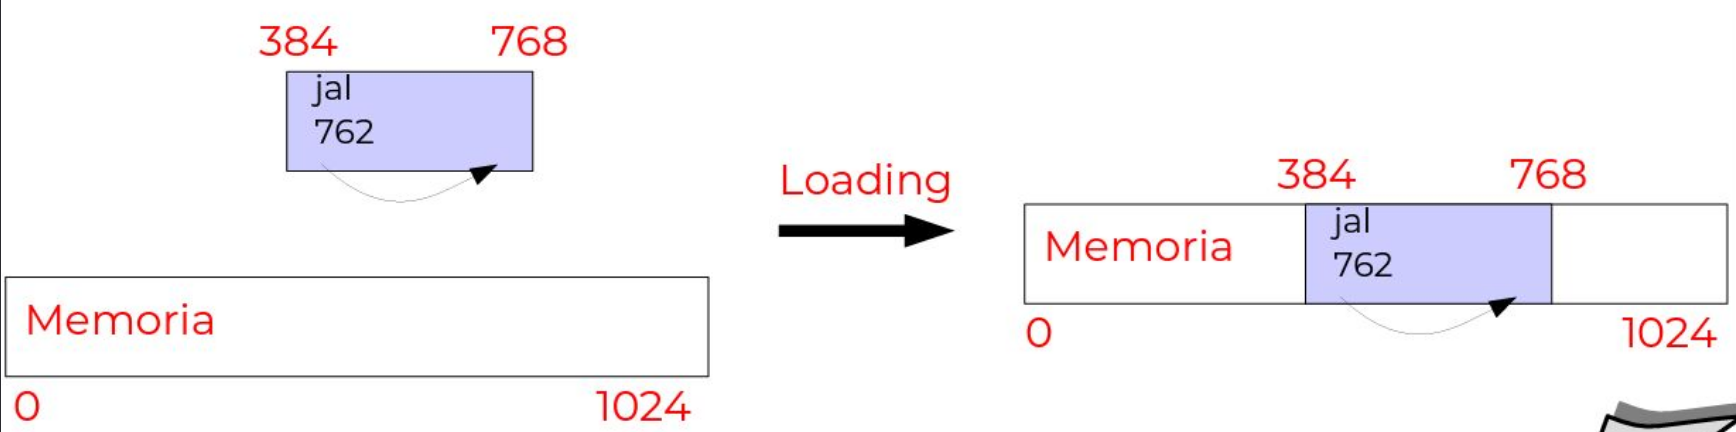
\includegraphics[width=0.7\linewidth]{Images/Screenshot 2025-01-16 at 18-28-27 so-05-memoria - so-05-memoria.pdf.png}
\end{figure}


\paragraph{Vantaggi:} non richiede hardware speciale, è semplice, molto veloce.
\paragraph{Svantaggi:} non funziona con la multiprogrammazione.

\subsubsection{Binding durante il caricamento}
Il codice generato dal compilatore non contiene indirizzi assoluti ma relativi (al PC oppure ad un indirizzo base), questo tipo di codice viene detto \textbf{rilocabile}.
Durante il caricamento il loader si preoccupa di aggiornare tutti i riferimenti agli indirizzi di memoria coerentemente al punto iniziale di caricamento.
\begin{figure} [h]
    \centering
    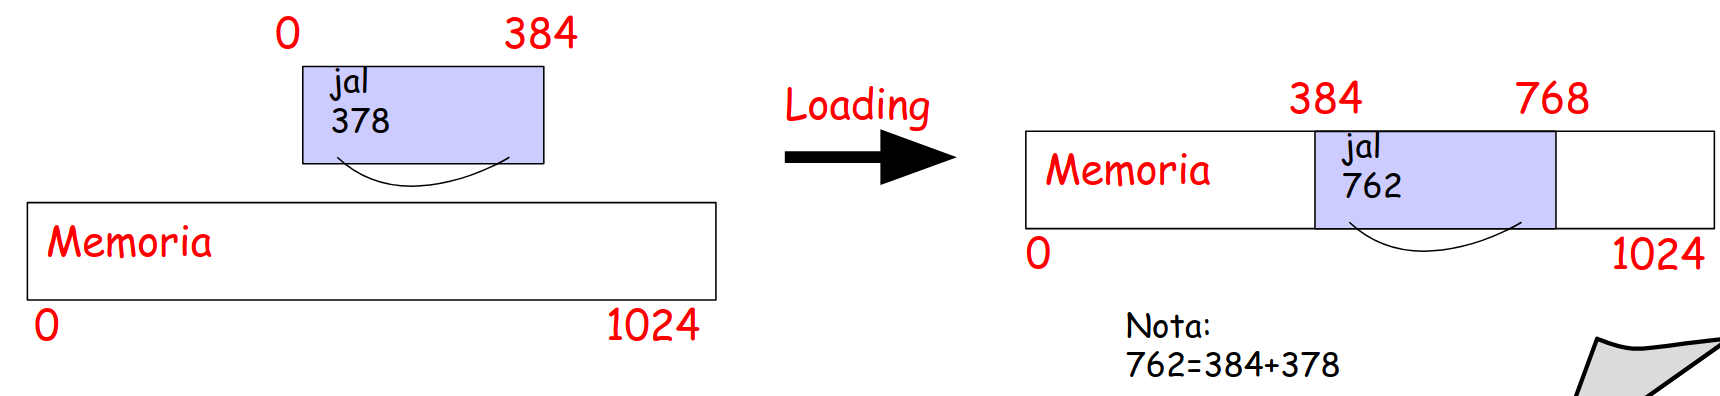
\includegraphics[width=0.7\linewidth]{Images/Screenshot 2025-01-16 at 18-30-35 so-05-memoria - so-05-memoria.pdf.png}
\end{figure}

\paragraph{Vantaggi:} permette di gestire multiprogrammazione, non richiede uso di hardware particolare.
\paragraph{Svantaggi:} richiede una traduzione degli indirizzi da parte del loader, e quindi formati particolari dei file eseguibili.

\subsubsection{Binding durante l'esecuzione}
L'individuazione dell'indirizzo di memoria effettivo viene effettuata durante l'esecuzione da un componente hardware apposito:
la memory management unit (\textbf{MMU}).

\begin{figure} [h]
    \centering
    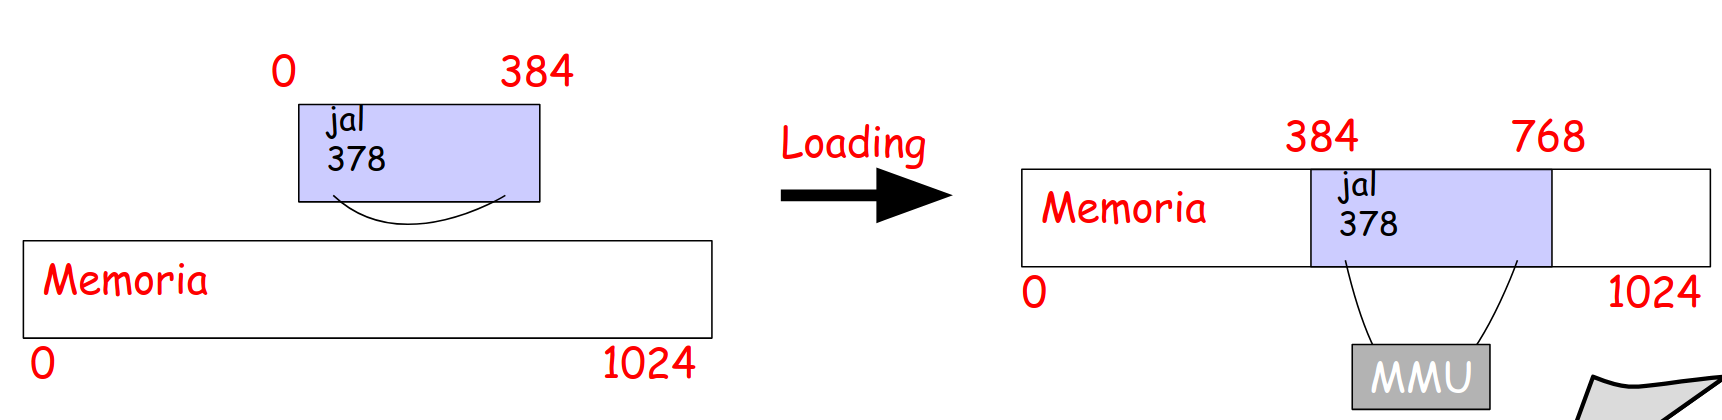
\includegraphics[width=0.7\linewidth]{Images/Screenshot 2025-01-16 at 18-33-56 so-05-memoria - so-05-memoria.pdf.png}
\end{figure}

\subsubsection{Indirizzi logici e indirizzi fisici}

\paragraph{Spazio di indirizzamento logico} ogni processo è associato ad uno spazio di indirizzamento logico, gli indirizzi usati in un processo sono indirizzi logici, ovvero riferimenti a
questo spazio di indirizzamento.

\paragraph{Spazio di indirizzamento fisico} ad ogni indirizzo logico corrisponde un indirizzo fisico, la MMU opera come una funzione di traduzione da indirizzi logici a indirizzi fisici.

\begin{figure} [h]
    \centering
    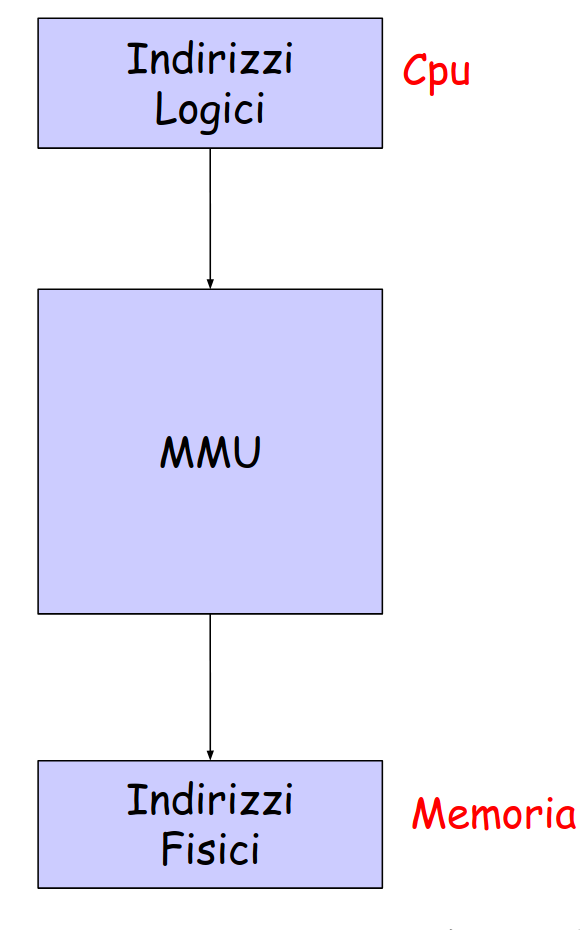
\includegraphics[width=0.25\linewidth]{Images/Screenshot 2025-01-16 at 18-40-39 so-05-memoria - so-05-memoria.pdf.png}
\end{figure}

\subsection{Loading Dinamico}
Il loading dinamico consente di poter caricare alcune routine di libreria solo quando vengono richiamate.
Tutte le routine a caricamento dinamico risiedono su un disco (codice rilocabile), quando servono vengono caricate, le routine poco utili \textit{(e.g., casi di errore rari...)} non vengono caricate in
memoria al caricamento dell'applicazione.

\textit{Nota: spetta al programmatore sfruttare questa possibilità, dato che il sistema operativo fornisce semplicemente una libreria che implementa le funzioni di caricamento dinamico.}


\subsection{Linking statico}
Se il linker collega e risolve tutti i riferimenti dei programmi, le routine di libreria vengono copiate in ogni programma che le usa
\textit{(e.g. printf in tutti i programmi C)}.

\subsection{Linking dinamico}
E' possibile posticipare il linking delle routine di libreria al momento del primo riferimento durante l'esecuzione.
Consente di avere eseguibili più compatti e le librerie vengono implementate come codice reentrant, ovvero esiste una sola istanza della libreria in memoria e tutti i programmi eseguono il codice di questa istanza.

\paragraph{Vantaggi:} risparmio di memoria, consente l'aggiornamento automatico delle versioni delle librerie
che vengono caricate alla successiva attivazione dei programmi.

\paragraph{Svantaggi:} può causare problemi di 'versioning', ovvero conflitti che si verificano quando diverse applicazioni richiedono versioni diverse della stessa libreria condivisa o quando l'aggiornamento di una libreria la rende incompatibile con alcune applicazioni che la utilizzano.
\newpage
\section{Allocazione}
\subsection{Definizioni}
E' una delle funzioni principali del gestore di memoria.
Consiste nel reperire ed assegnare uno spazio di memoria fisica  a un programma che viene attivato, oppure per soddisfare ulteriori richieste effettuate dai programmi durante la loro esecuzione.

\paragraph{Allocazione contigua} tutto lo spazio assegnato ad un programma deve essere formato da celle consecutive.
\paragraph{Allocazione non contigua} è possibile assegnare a un programma aree di memorie separate.

\textit{Nota: la MMU deve essere in grado di gestire la conversione degli indirizzi in modo coerente. Esempio: la MMU basata su rilocazione gestisce solo allocazione contigua.}

\paragraph{Allocazione statica:} un programma deve mantenere la propria area di memoria dal caricamento alla terminazione. Non è possibile rilocare il programma durante l'esecuzione.
\paragraph{Allocazione dinamica:} durante l'esecuzione, un programma può essere spostato all'interno della memoria.

\subsection{Allocazione a partizioni fisse}
\paragraph{Descrizione:} la memoria disponibile (quella non occupata dal s.o.) viene suddivisa in partizioni, ogni processo viene caricato in una delle partizioni libere che ha dimensione sufficiente a contenerlo.

\paragraph{Caratteristiche:} statica e contigua. Molto semplice.
Ma produce spreco di memoria e ha un grado di parallelismo limitato dal numero di partizioni.

\begin{figure} [h]
    \centering
    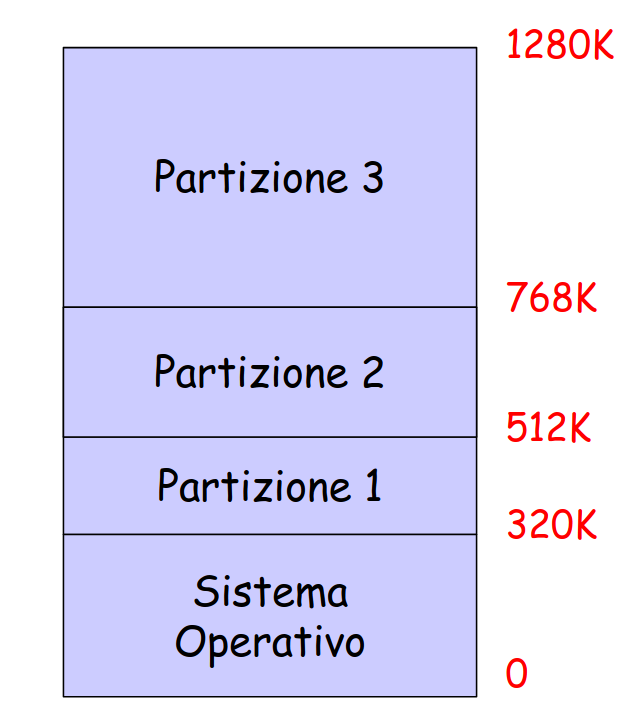
\includegraphics[width=0.3\linewidth]{Images/Screenshot 2025-01-16 at 19-02-29 so-05-memoria - so-05-memoria.pdf.png}
\end{figure}

E' possibile utilizzare una coda per partizione, oppure una coda
comune per tutte le partizioni. Esiste una sola partizione,
dove viene caricato un unico programma utente.

\subsubsection{Frammentazione interna}
Nell'allocazione a partizione fisse se un processo occupa una dimensione inferiore a quella della partizione che lo
contiene, lo spazio non utilizzato è sprecato.

La presenza di spazio inutilizzato all'interno di un'unità di allocazione si chiama frammentazione interna.

\textit{Nota: il fenomeno della frammentazione interna
non è limitata all'allocazione a partizioni fisse, ma è generale
a tutti gli approcci in cui è possibile allocare più memoria di
quanto richiesto (per motivi di organizzazione).}

\begin{figure} [h]
    \centering
    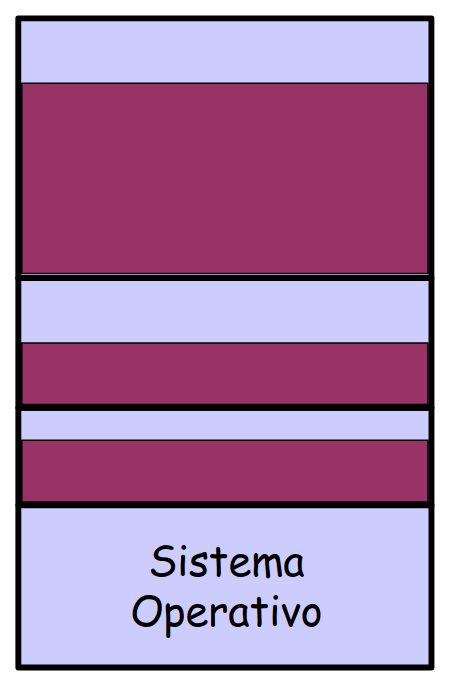
\includegraphics[width=0.22\linewidth]{Images/Screenshot 2025-01-16 at 19-06-25 so-05-memoria - so-05-memoria.pdf.png}
\end{figure}
\newpage
\subsection{Allocazione a partizioni dinamiche}

\paragraph{Descrizione:} la memoria disponibile viene assegnata ai processi che ne fanno richiesta.
Nella memoria possono essere presenti diverse zone inutilizzate per effetto della terminazione di processi, oppure per non completo utilizzo dell'area disponibile da parte dei processi
attivi.

\paragraph{Caratteristiche:} statica e contigua. Esistono diverse politiche per la scelta dell'area da utilizzare.
\begin{figure} [h]
    \centering
    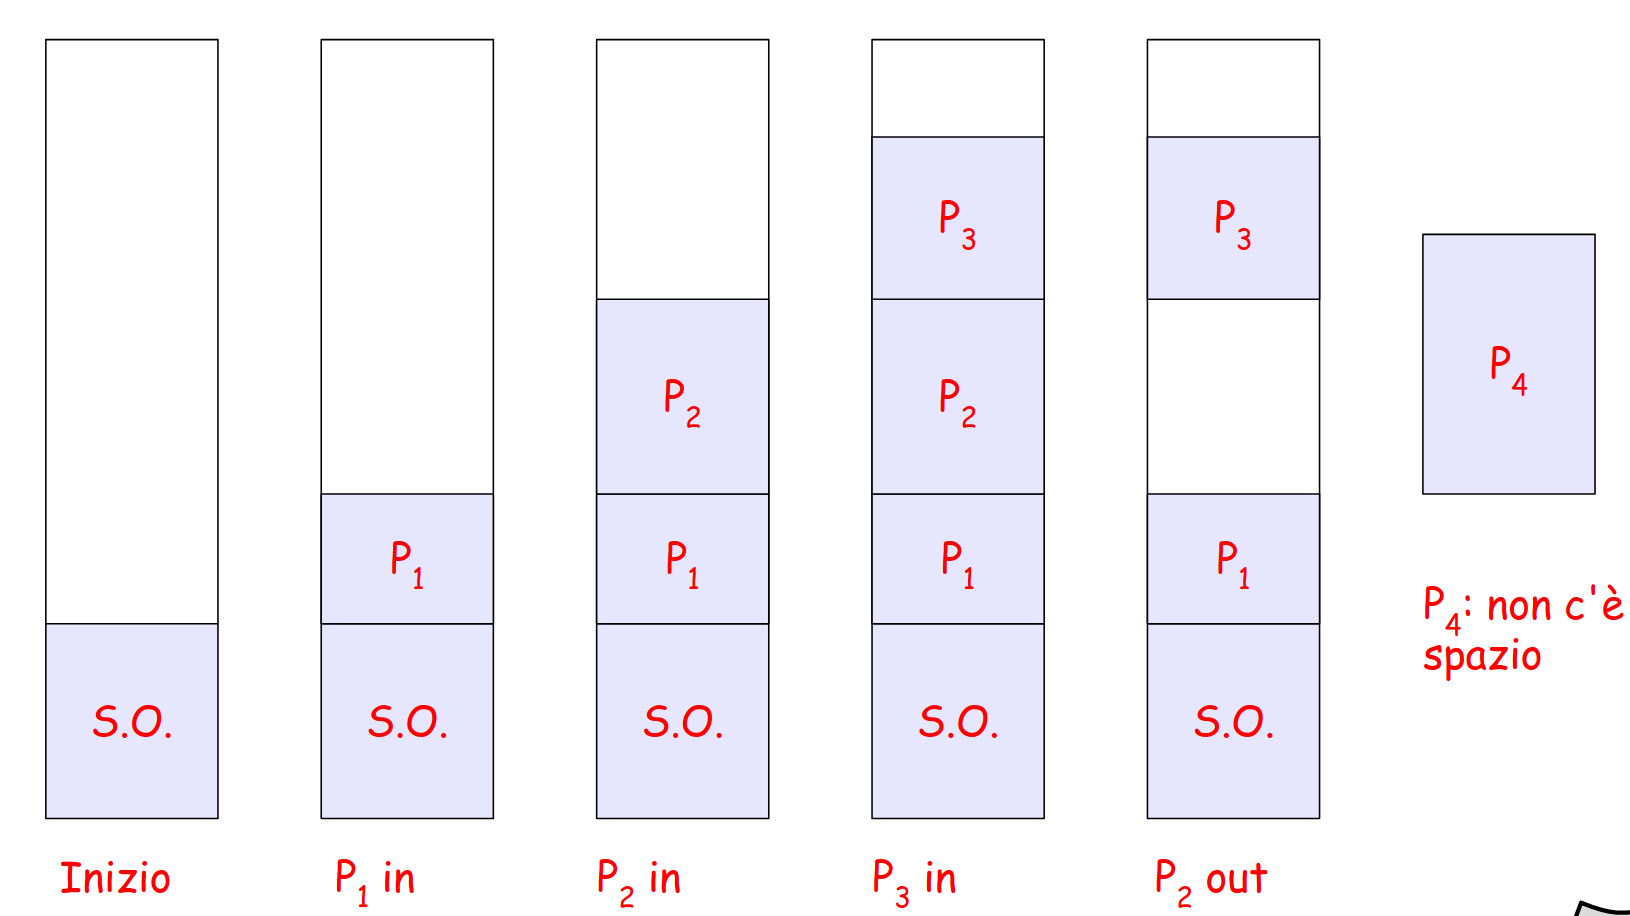
\includegraphics[width=0.6\linewidth]{Images/Screenshot 2025-01-16 at 19-10-01 so-05-memoria - so-05-memoria.pdf.png}
\end{figure}


\subsubsection{Frammentazione esterna}
Dopo un certo numero di allocazioni e deallocazioni di memoria dovute all'attivazione e alla terminazione dei processi lo spazio libero appare suddiviso in piccole aree questo fenomeno prende il nome di frammentazione esterna.

\textit{Nota: la frammentazione interna dipende dall'uso di unità di allocazione di dimensione diversa da quella richiesta.}


\subsection{Compattazione}
Se è possibile rilocare i programmi durante la loro esecuzione,
è allora possibile procedere alla compattazione della memoria.
Compattare la memoria significa spostare in memoria tutti i programmi in modo da riunire tutte le aree inutilizzate, è un’operazione volta a risolvere il problema della frammentazione esterna. 

Purtroppo è un’operazione molto onerosa in quanto occorre copiare (fisicamente) in memoria grandi quantità di dati.
Non può essere utilizzata in sistemi interattivi dato che i processi devono essere fermi durante la compattazione.

\begin{figure} [h]
    \centering
    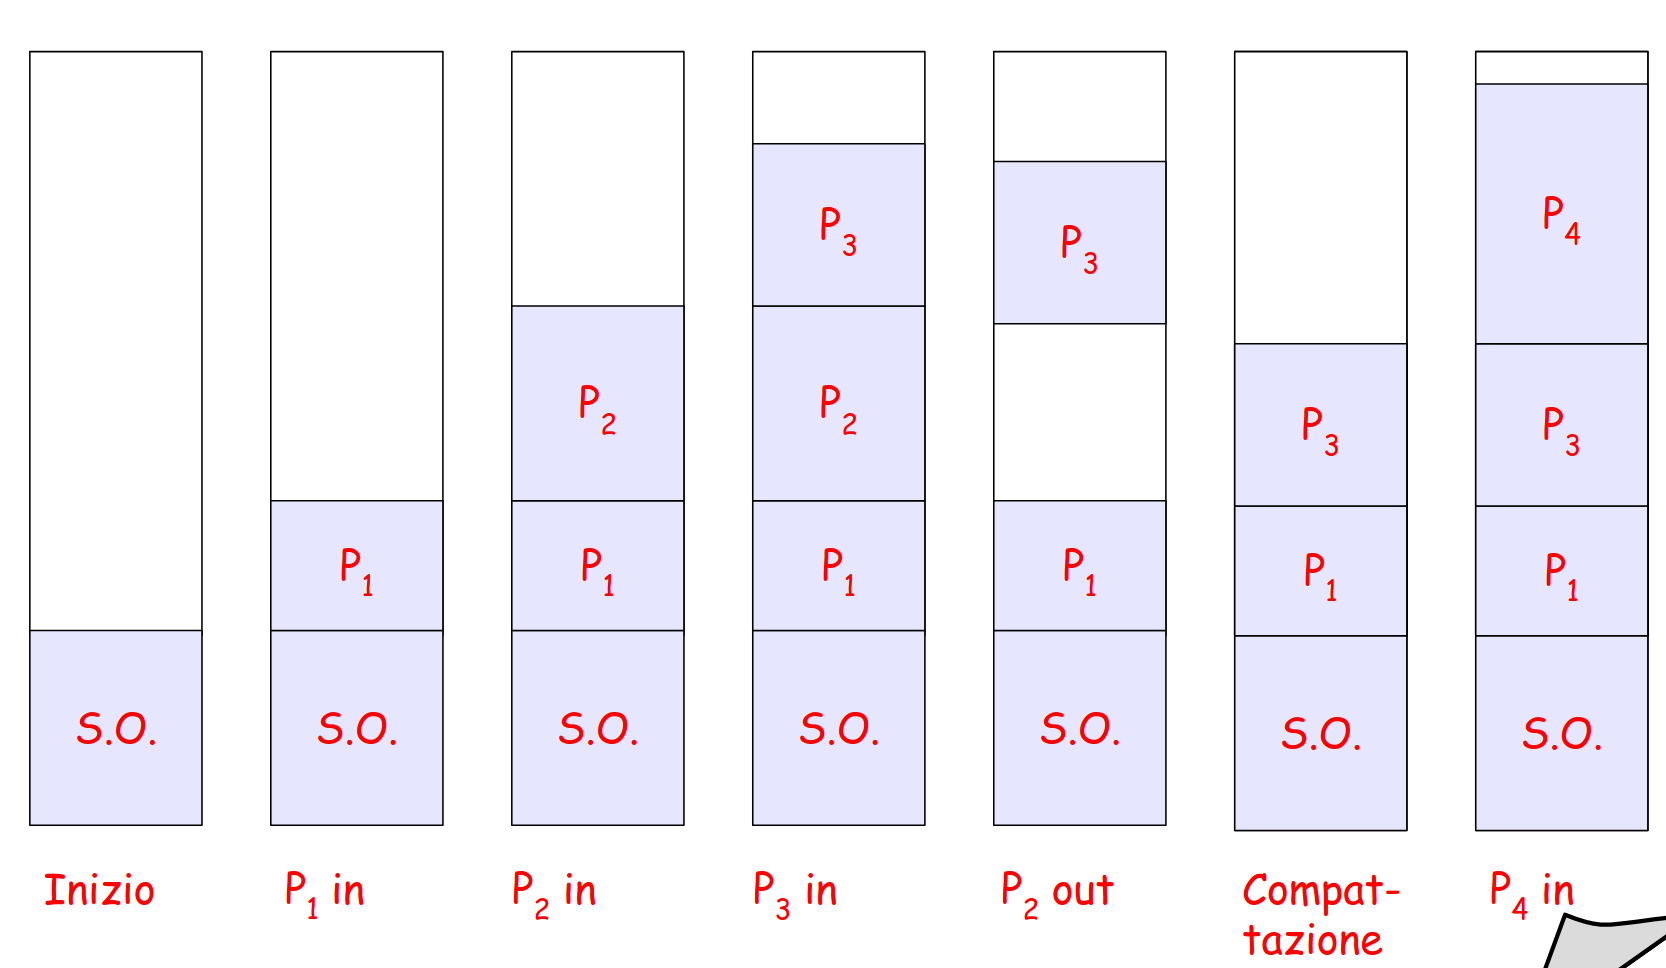
\includegraphics[width=0.6\linewidth]{Images/Screenshot 2025-01-16 at 19-21-10 so-05-memoria - so-05-memoria.pdf.png}
\end{figure}

Quando la memoria è assegnata dinamicamente abbiamo bisogno di una struttura dati per mantenere informazioni sulle zone
libere e sulle zone occupate, le strutture dati possibili: mappe di bit, liste con puntatori, ...
\newpage
\subsubsection{Mappa di bit}
La memoria viene suddivisa in unità di allocazione dove ad ogni unità di allocazione corrisponde un bit in una bitmap. Le unità libere sono associate ad un bit di valore 0, le unità occupate sono
associate ad un bit di valore 1.

\begin{figure} [h]
    \centering
    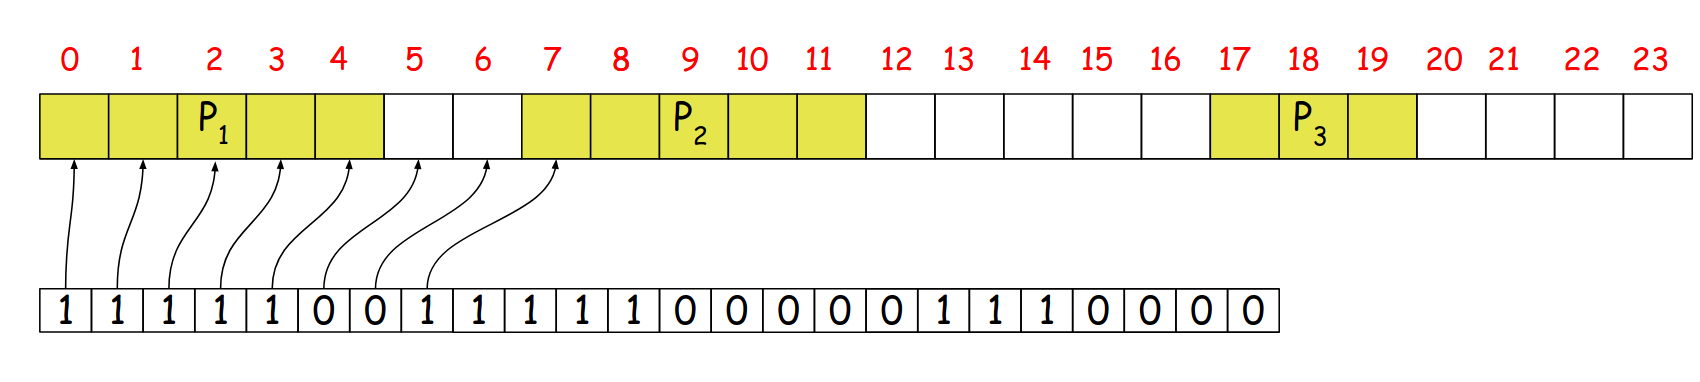
\includegraphics[width=0.7\linewidth]{Images/Screenshot 2025-01-17 at 15-29-40 so-05-memoria - so-05-memoria.pdf.png}
\end{figure}

La dimensione dell'unità di allocazione è un parametro importante
dell'algoritmo, esistte un trade-off fra dimensione della bitmap e frammentazione interna.
\paragraph{Vantaggi:} la struttura dati ha una dimensione fissa e calcolabile a priori.
\paragraph{Svantaggi:} per individuare uno spazio di memoria di dimensione \textbf{k} unità, è necessario
cercare una sequenza di \textbf{k} bit 0 consecutivi, in generale, tale operazione è \textbf{O(m)}, dove \textbf{m} rappresenta il numero di unità di
allocazione.

\subsubsection{Liste di puntatori}

Si mantiene una lista dei blocchi allocati e liberi di memoria, ogni elemento della lista specifica, se si tratta di un processo (P) o di un blocco libero (hole, H), la dimensione (inizio/fine) del segmento.

\begin{figure} [h]
    \centering
    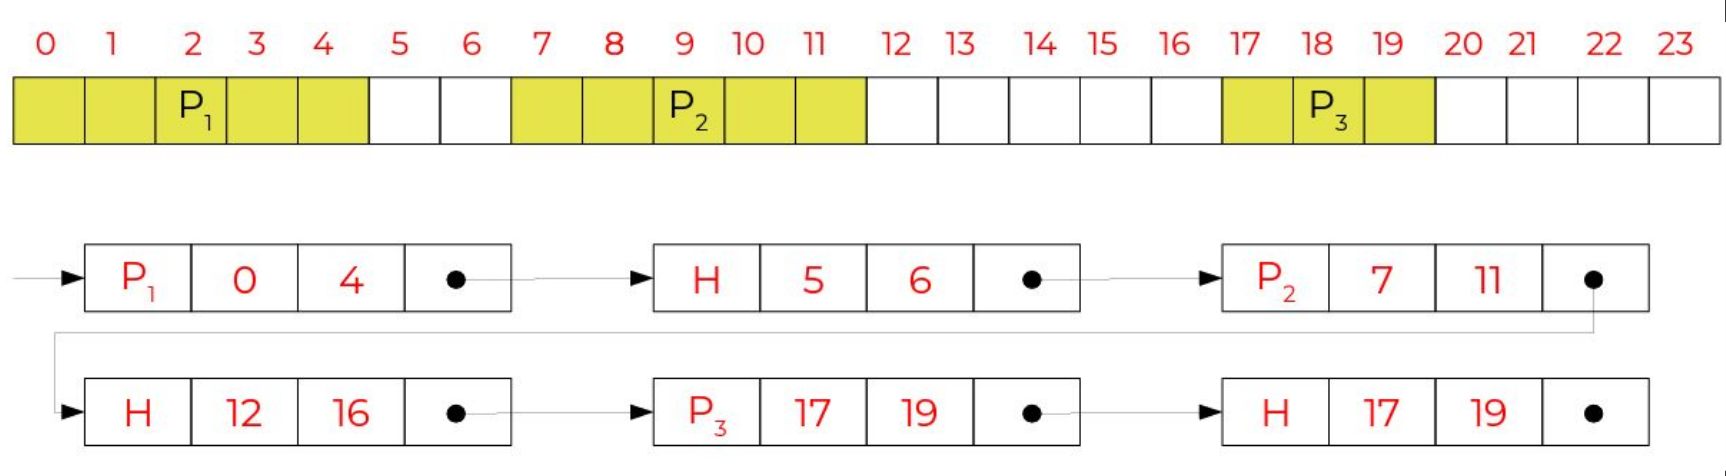
\includegraphics[width=0.7\linewidth]{Images/Screenshot 2025-01-17 at 15-32-58 so-05-memoria - so-05-memoria.pdf.png}
\end{figure}

Un blocco libero viene selezionato e suddiviso in due parti:
\begin{enumerate}
    \item un blocco processo della dimensione desiderata
    \item un blocco libero con quanto rimane del blocco iniziale
\end{enumerate}

\paragraph{Allocazione di memoria}
Se la dimensione del processo è uguale a quella del blocco scelto, si crea solo un nuovo blocco processo.
\begin{figure} [h]
    \centering
    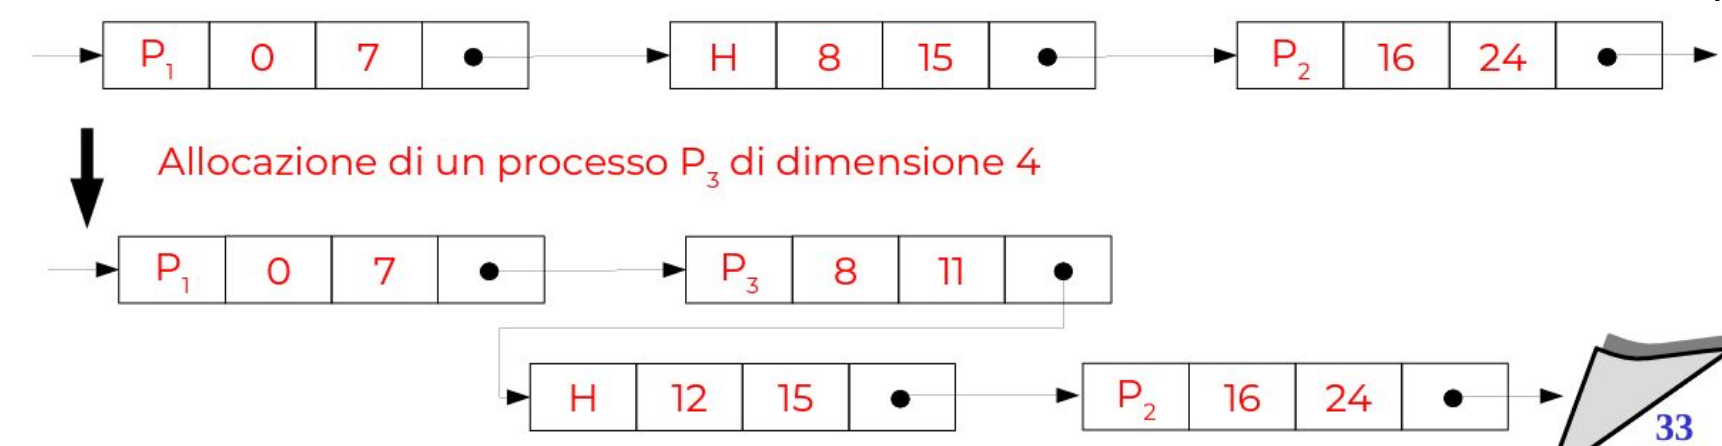
\includegraphics[width=0.7\linewidth]{Images/Screenshot 2025-01-17 at 15-35-24 so-05-memoria - so-05-memoria.pdf.png}
\end{figure}

\paragraph{Deallocazione di memoria}
A seconda dei blocchi vicini, lo spazio liberato può creare un nuovo blocco libero, oppure essere accorpato ai blocchi vicini.
L'operazione può essere fatta in tempo O(1).

\begin{figure} [h]
    \centering
    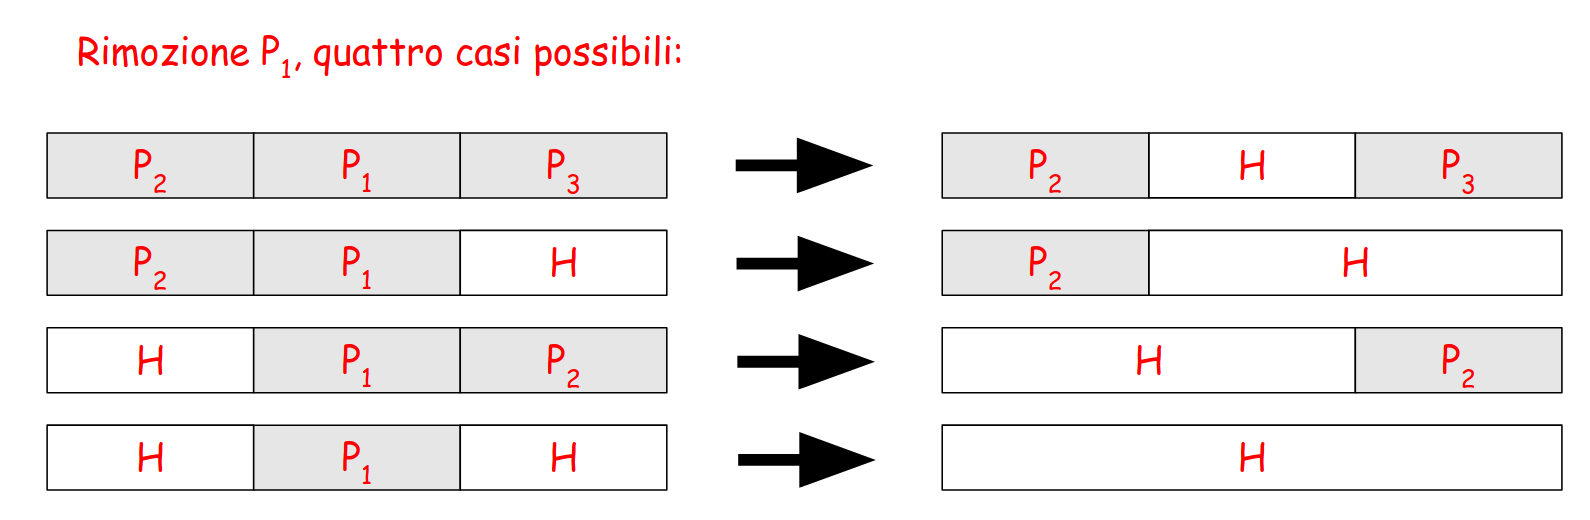
\includegraphics[width=0.7\linewidth]{Images/Screenshot 2025-01-17 at 15-37-05 so-05-memoria - so-05-memoria.pdf.png}
\end{figure}

\paragraph{Selezione blocco libero}
L'operazione di selezione di un blocco libero è concettualmente
indipendente dalla struttura dati.
\begin{itemize}
    \item \textbf{First Fit}: scorre la lista dei blocchi liberi fino a quando non trova il primo segmento vuoto grande abbastanza da contenere il processo.
    \item \textbf{Next Fit}: come First Fit, ma invece di ripartire sempre dall'inizio, parte dal punto dove si era fermato all'ultima allocazione (è stato progettato per evitare di frammentare continuamente l'inizi della memoria ma sorprendentemente, ha performance peggiori di First Fit).
    \item \textbf{Best Fit}: seleziona il più piccolo fra i blocchi liberi presenti in memoria. Più lento di First Fit, in quanto richiede di esaminare tutti i blocchi liberi presenti in memoria, genera più frammentazione di First Fit, in quanto tende a riempire la memoria di blocchi liberi troppo piccoli.
    \item \textbf{Worst fit}: seleziona il più grande fra i blocchi liberi presenti in memoria. Proposto per evitare i problemi di frammentazione di First/Best Fit, rende difficile l'allocazione di processi di grosse dimensioni.
\end{itemize}

Nella struttura proposta liste di puntatori, il costo della deallocazione è O(1).
Possibile ottimizzare il costo di allocazione mantenendo una lista di blocchi liberi separata o eventualmente, ordinando tale lista per dimensione.

\newpage


\section{Paginazione}
\subsection{Introduzione}
I meccanismi visti (partizioni fisse, partizioni dinamiche) non sono efficienti nell'uso della memoria perchè causano le frammentazioni.

La paginazione è l'approccio contemporaneo che riduce il fenomeno di frammentazione interna ed elimina il fenomeno della frammentazione esterna.

Lo spazio di indirizzamento logico di un processo viene suddiviso in un insieme di blocchi di dimensione fissa chiamati
\textbf{pagine}.

La memoria fisica  viene suddivisa in un insieme di blocchi della stessa dimensione delle pagine, chiamati \textbf{frame}.

Quando un processo viene allocato in memoria: vengono reperiti ovunque in memoria un numero sufficiente di frame per contenere le pagine del processo.

\begin{figure} [h]
    \centering
    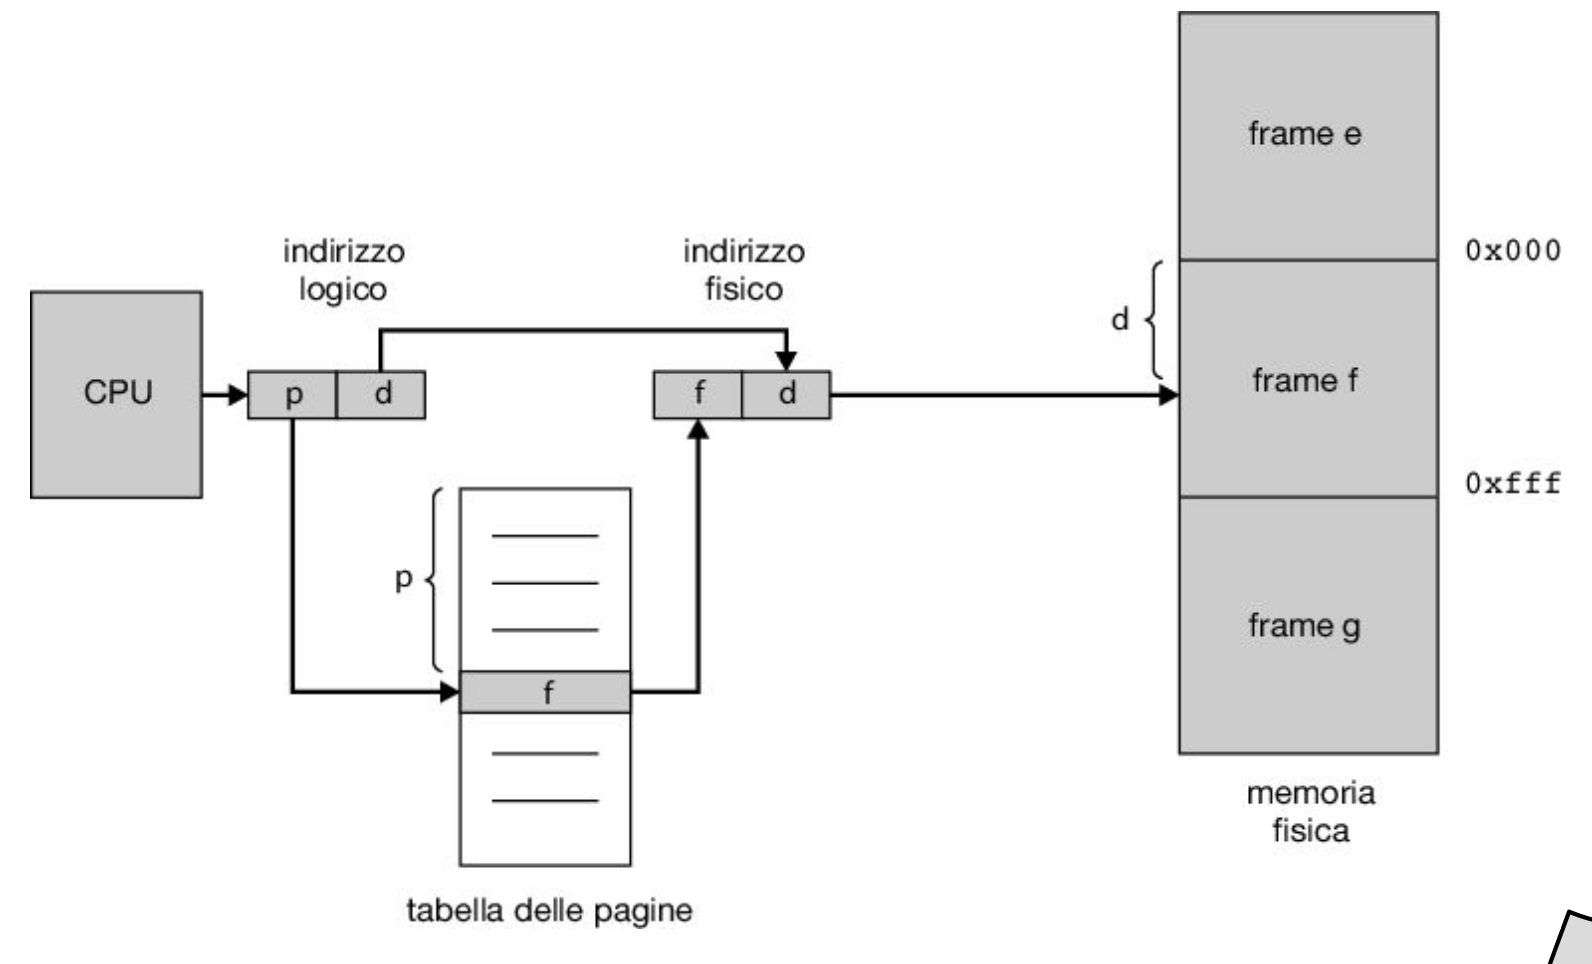
\includegraphics[width=0.7\linewidth]{Images/Screenshot 2025-01-17 at 15-53-05 so-05-memoria - so-05-memoria.pdf.png}
\end{figure}

\begin{figure} [h]
    \centering
    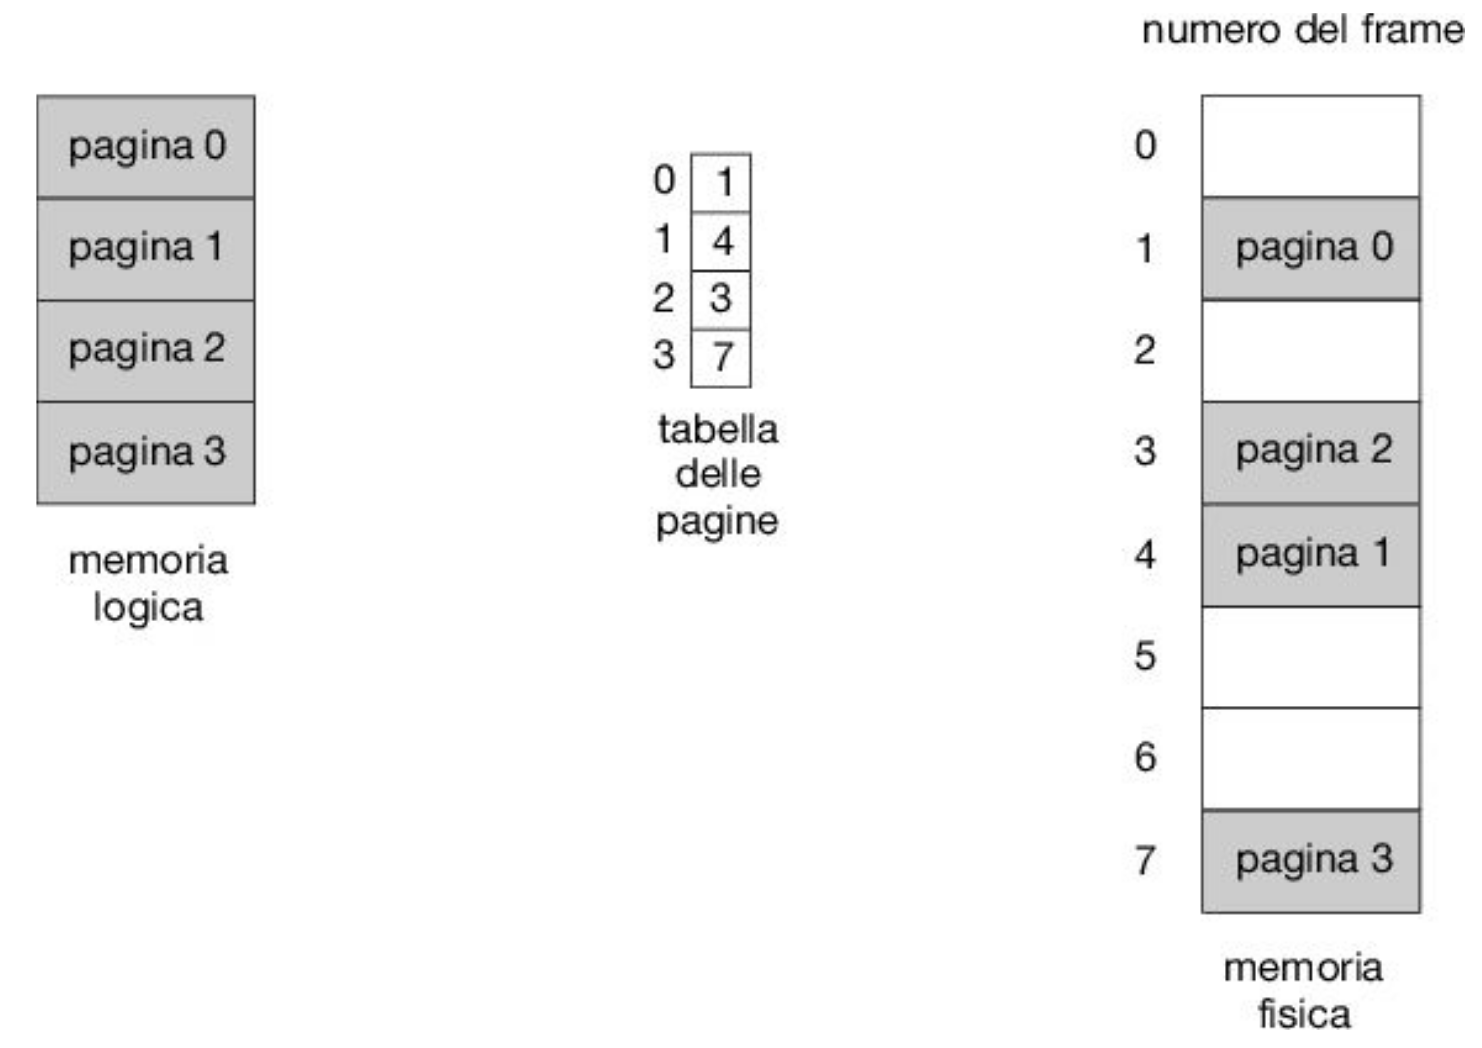
\includegraphics[width=0.7\linewidth]{Images/Screenshot 2025-01-17 at 15-54-41 so-05-memoria - so-05-memoria.pdf.png}
\end{figure}

\begin{figure} [h]
    \centering
    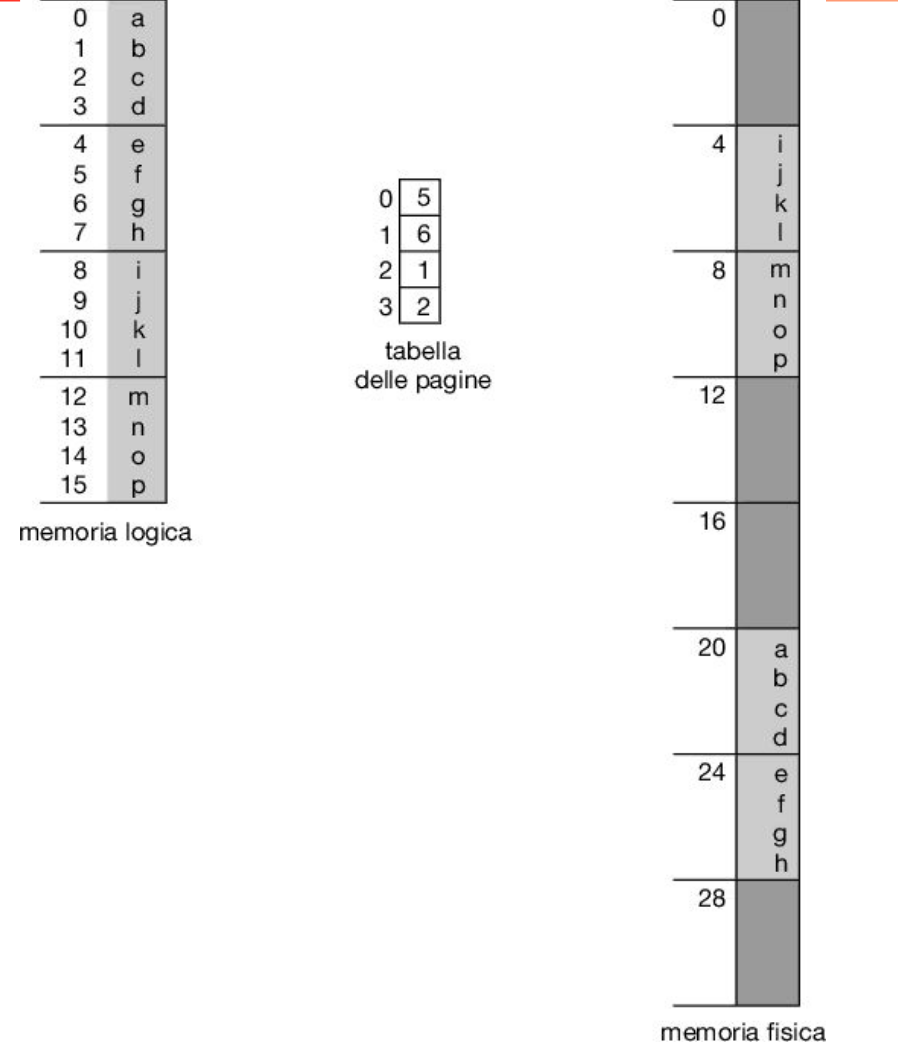
\includegraphics[width=0.5\linewidth]{Images/Screenshot 2025-01-17 at 15-56-06 so-05-memoria - so-05-memoria.pdf.png}
\end{figure}
\newpage
\paragraph{Dimensione delle pagine}
La dimensione delle pagine deve essere una potenza di due, per
semplificare la trasformazione da indirizzi logici a indirizzi fisici, la scelta della dimensione deriva da un trade-off poichè con pagine troppo piccole, la tabella delle pagine cresce di
dimensioni mentre con pagine troppo grandi, lo spazio di memoria perso per frammentazione interna può essere considerevole.
\textit{(valori tipici: 1KB, 2KB, 4KB)}

\subsubsection{Implementazione della page table}
Dove mettere la tabella delle pagine?
\paragraph{Soluzione 1:} registri dedicati. La tabella può essere contenuta in un insieme di registri ad alta velocità all'interno del modulo MMU (o della CPU), però è una soluzione troppo costosa.

\paragraph{Soluzione 2:} totalmente in memoria. Il problema è che il numero di accessi in memoria verrebbe raddoppiato; ad
ogni riferimento, bisognerebbe prima accedere alla tabella delle
pagine, poi al dato.

\subsection{Translation lookaside buffer (TLB)}
\paragraph{Descrizione:} un \textbf{TLB} è costituito da un insieme di registri associativi ad alta velocità. Ogni registro è suddiviso in due parti, una chiave e un valore.
Quando avviene l'operazione di \textbf{lookup}: viene richiesta la ricerca di una chiave che viene confrontata simultaneamente con tutte le chiavi presenti nel buffer.
\begin{itemize}
    \item se la chiave è presente (\textbf{TLB hit}), si ritorna il valore
corrispondente.
    \item se la chiave non è presente (\textbf{TLB miss}), si utilizza la tabella in memoria.
\end{itemize}

\begin{figure} [h]
    \centering
    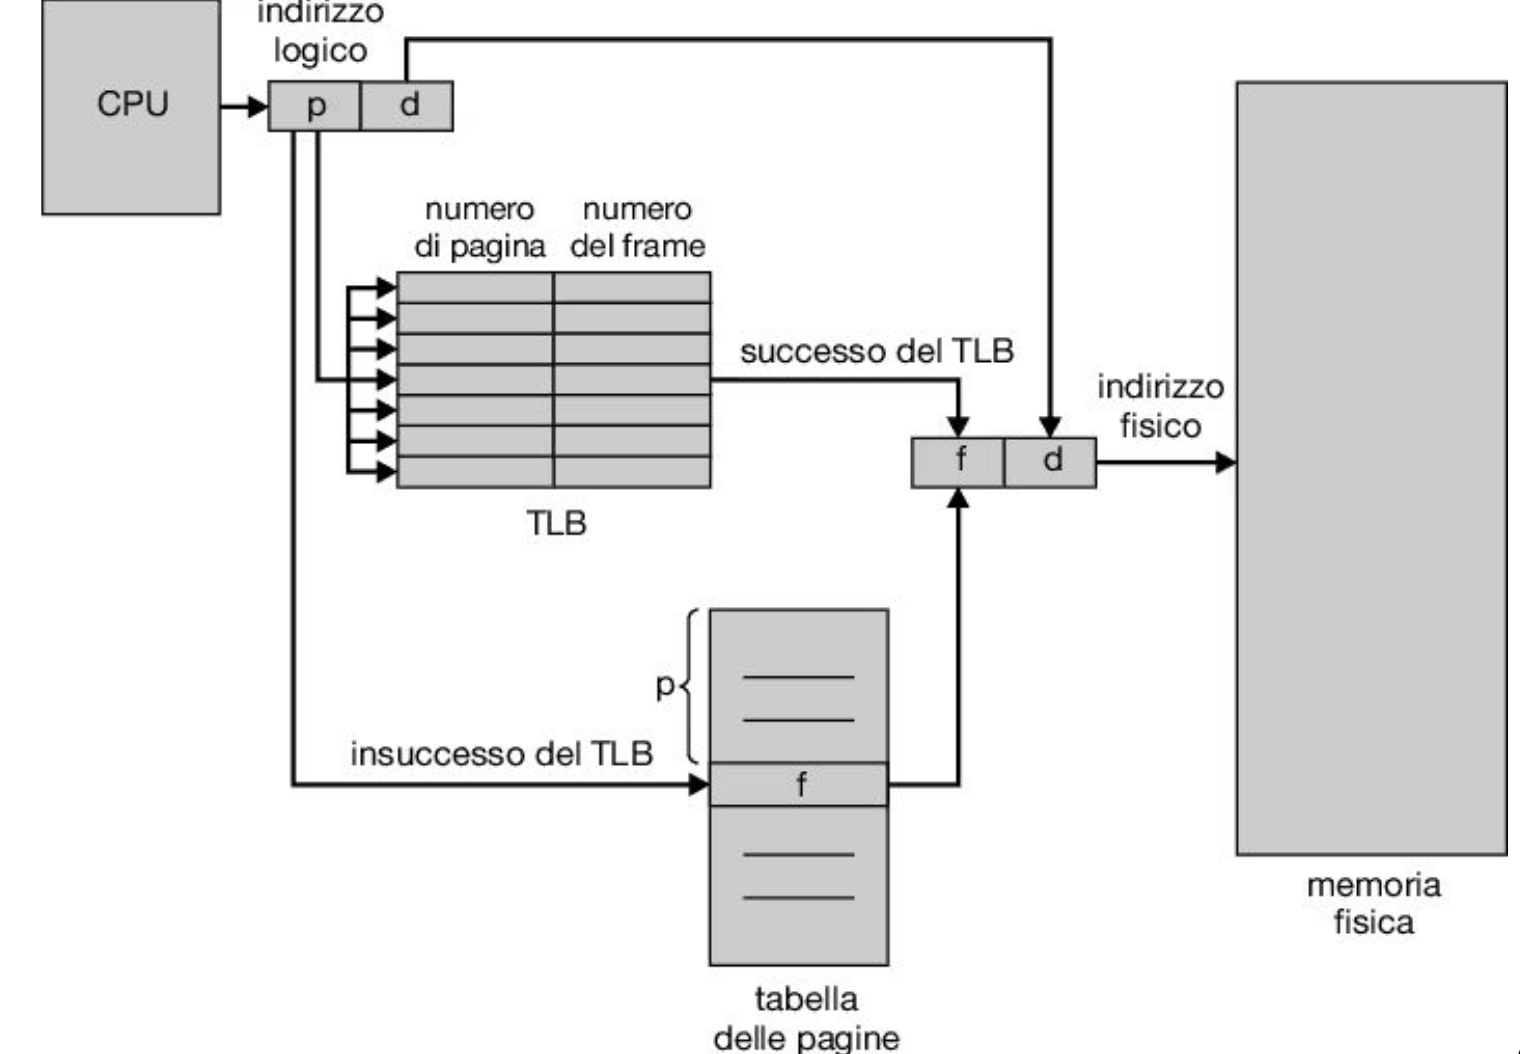
\includegraphics[width=0.7\linewidth]{Images/Screenshot 2025-01-17 at 16-06-35 so-05-memoria - so-05-memoria.pdf.png}
\end{figure}

\newpage
\section{Segmentazione}
\subsection{Introduzione e confronti}
In un sistema basato su segmentazione, uno spazio di indirizzamento logico è dato da un insieme di segmenti.

Un \textbf{segmento} è un'area di memoria (logicamente continua)
contenente elementi tra loro affini dove ogni segmento è caratterizzato da un nome (normalmente un indice)
e da una lunghezza.

Ogni riferimento di memoria è dato da una coppia \textit{(nome segmento, offset)}.

\subsubsection{Segmentazione vs Paginazione}
\paragraph{Paginazione:}
\begin{itemize}
    \item la divisione in pagine è automatica.
    \item  le pagine hanno dimensione fissa.
    \item le pagine possono contenere informazioni disomogenee (\textit{ad es. sia codice sia dati)}.
    \item una pagina ha un indirizzo.
    \item dimensione tipica della pagina: 1-4 KB.
\end{itemize}

\paragraph{Segmentazione:}

\begin{itemize}
    \item la divisione in segmenti spetta al programmatore.
    \item  i segmenti hanno dimensione variabile.
    \item un segmento contiene informazioni omogenee per tipo di accesso e permessi di condivisione.
    \item un segmento ha un nome.
    \item dimensione tipica di un segmento: 64KB - 1MB.
\end{itemize}

\subsubsection{Segmentazione - condivisione}
La segmentazione consente la condivisione di codice e dati.

\textit{Esempio: editor condiviso}

\begin{figure} [h]
    \centering
    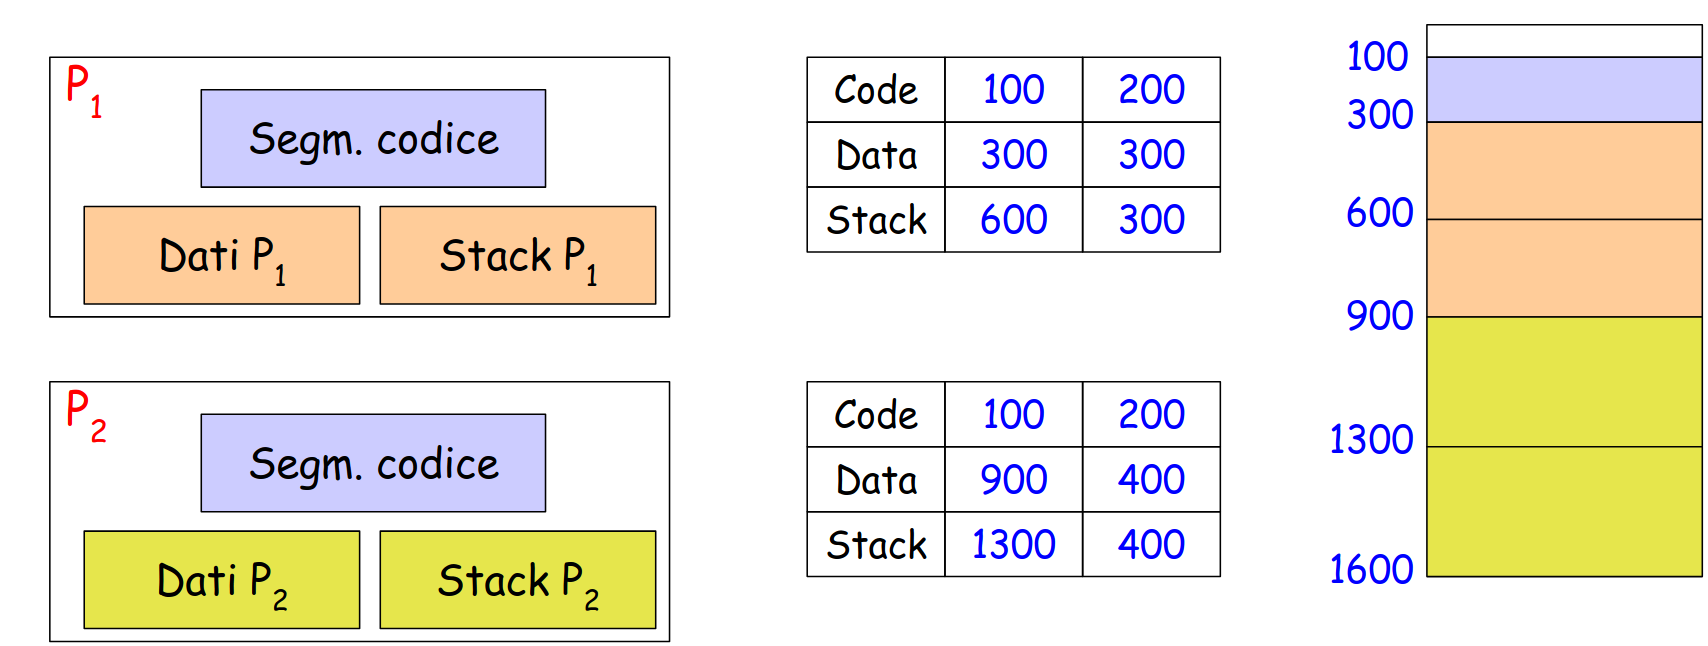
\includegraphics[width=0.7\linewidth]{Images/Screenshot 2025-01-17 at 16-16-13 so-05-memoria - so-05-memoria.pdf.png}
\end{figure}

\subsubsection{Segmentazione - frammentazione}
Allocare segmenti di dimensione variabile è del tutto equivalente
al problema di allocare in modo contiguo la memoria dei
processi. E' possibile utilizzare  tecniche di allocazione dinamica (e.g., First Fit), compattazione, ma così torniamo ai problemi precedenti.

\subsubsection{Segmentazione - paginazione}
E' possibile utilizzare il metodo della paginazione combinato al metodo della segmentazione, ogni segmento viene suddiviso in pagine che vengono allocate in frame liberi della memoria (non necessariamente contigui).

\paragraph{Requisiti hardware:} la MMU deve avere sia il supporto per la segmentazione sia il supporto per la paginazione.
\paragraph{Benefici:} sia quelli della segmentazione (condivisione, protezione) e sia quelli della paginazione (no frammentazione esterna).

\newpage

\section{Memoria virtuale}
\subsection{Introduzione}
\paragraph{Definizione:} è la tecnica che permette l'esecuzione di processi che non sono completamente in memoria.

Permette di eseguire in concorrenza processi che nel loro
complesso (o anche singolarmente) hanno necessità di memoria
maggiore di quella disponibile. La memoria virtuale può diminuire le prestazioni di un sistema se implementata (e usata) nel modo sbagliato.

Le istruzioni da eseguire e i dati su cui operano devono essere in memoria, ma non è necessario che l'intero spazio di indirizzamento logico di un processo sia in memoria. I processi non utilizzano tutto il loro spazio di indirizzamento contemporaneamente.

\paragraph{Implementazione:}
ogni processo ha accesso ad uno \textbf{spazio di indirizzamento virtuale} che può essere più grande di quello fisico. 

Gli indirizzi virtuali possono essere mappati su indirizzi fisici della memoria principale oppure, possono essere mappati su memoria secondaria, in questo caso: i dati associati vengono trasferiti in memoria principale, se la memoria è piena, si sposta in memoria secondaria i dati contenuti in memoria principale che sono considerati meno utili.

\paragraph{}
Si utilizza la tecnica della paginazione a richiesta (\textbf{demand paging}), ammettendo però che alcune pagine possano essere in memoria secondaria.

Nella tabella delle pagine si utilizza un bit (\textbf{v}, per valid) che indica se la pagina è presente in memoria centrale oppure no.

Quando un processo tenta di accedere ad un pagina non in
memoria il processore genera un trap (\textbf{page fault}) e un componente del s.o. (\textbf{pager}) si occupa di caricare la pagina mancante in memoria, e di aggiornare di conseguenza la tabella delle pagine.

\begin{figure} [h]
    \centering
    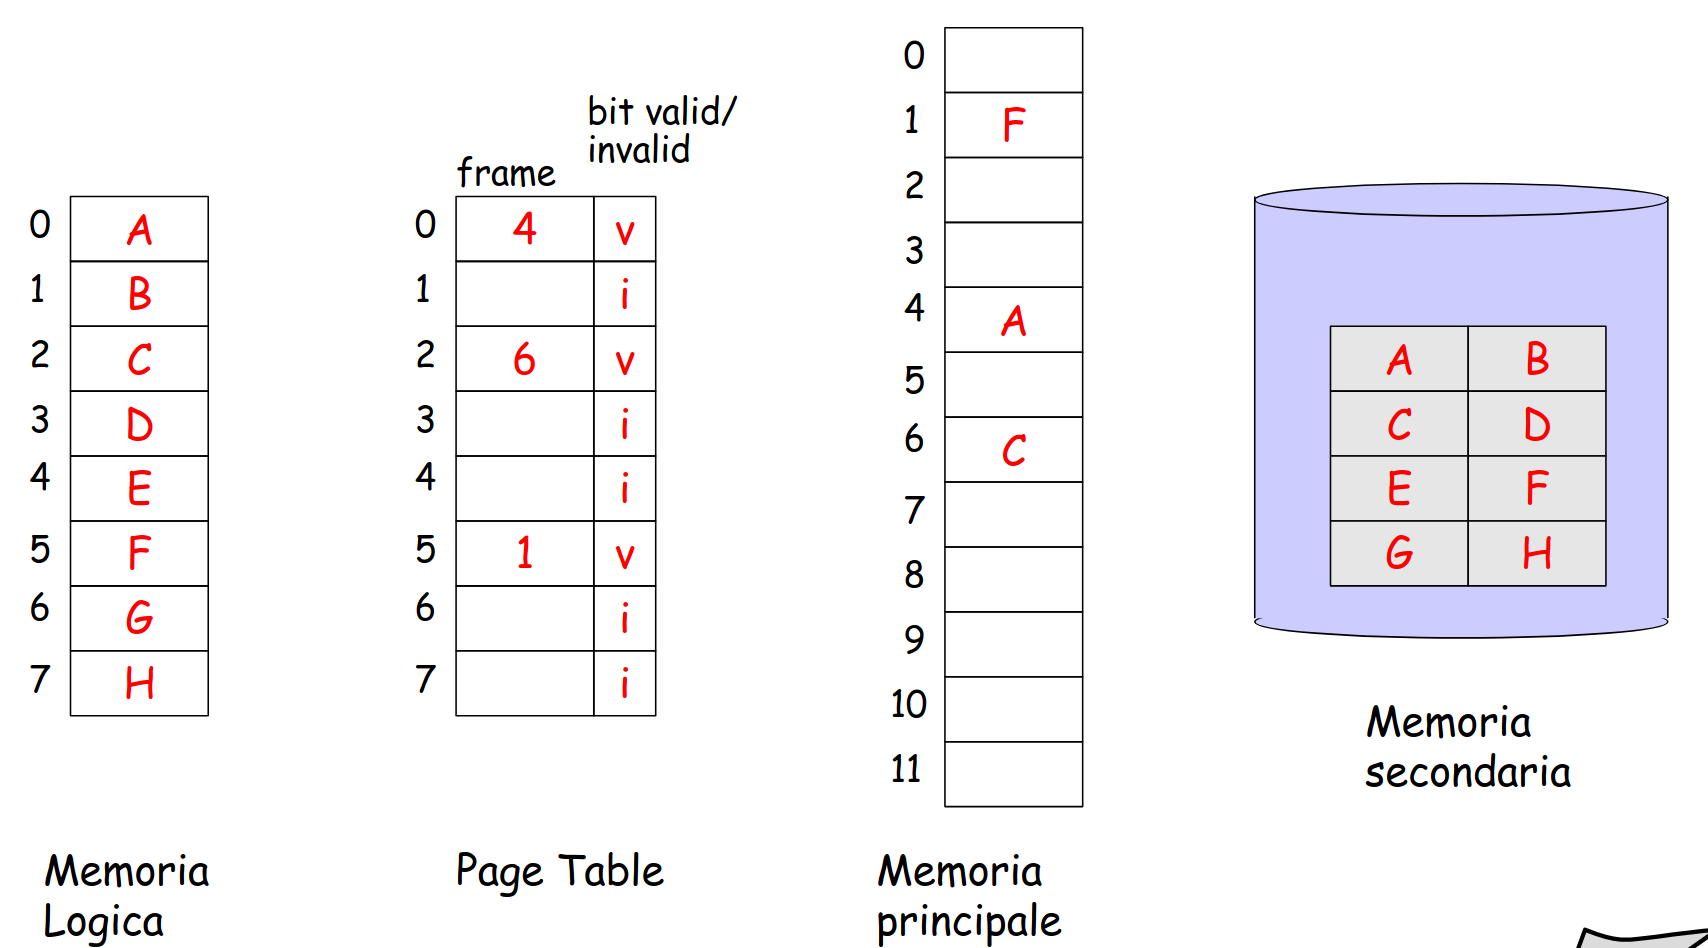
\includegraphics[width=0.7\linewidth]{Images/Screenshot 2025-01-17 at 16-42-29 so-05-memoria - so-05-memoria.pdf.png}
\end{figure}

\subsection{Pager/swapper}

\paragraph{Swap:} con questo termine si intende l'azione di copiare l'intera area di memoria usata da un processo. Era una tecnica utilizzata nel passato quando demand paging non esisteva.
\begin{itemize}
    \item dalla memoria secondaria alla memoria principale (\textbf{swap-in})
    \item dalla memoria principale alla memoria secondaria (\textbf{swap-out}).
\end{itemize}

La paginazione su richiesta (demand paging) può essere vista come una tecnica di swap di tipo lazy, viene caricato solo ciò che serve.

Per questo motivo alcuni sistemi operativi indicano il pager con il nome di \textbf{swapper} ma è da considerarsi una terminologia obsoleta.

Noi utilizziamo il termine s\textbf{wap area} per indicare l'area del disco
utilizzata per ospitare le pagine in memoria secondaria.
\newpage
\subsection{Gestione dei page fault}
Vediamo passo a passo come viene gestito il page fault:

1. Supponiamo che il codice in pagina 0 faccia riferimento alla pagina 1.
    \begin{figure} [h]
        \centering
        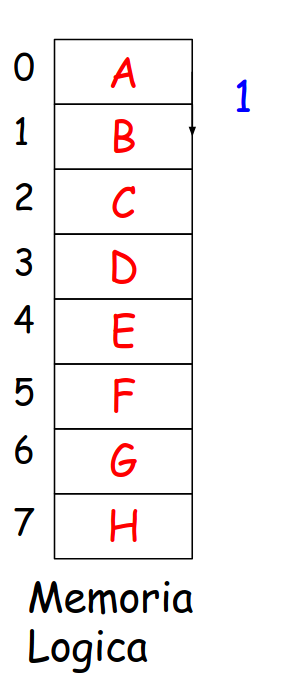
\includegraphics[width=0.1\linewidth]{Images/Screenshot 2025-01-17 at 16-49-22 so-05-memoria - so-05-memoria.pdf.png}
    \end{figure}
    
2. La MMU scopre che la pagina 1 non è in memoria principale.
    \begin{figure} [h]
        \centering
        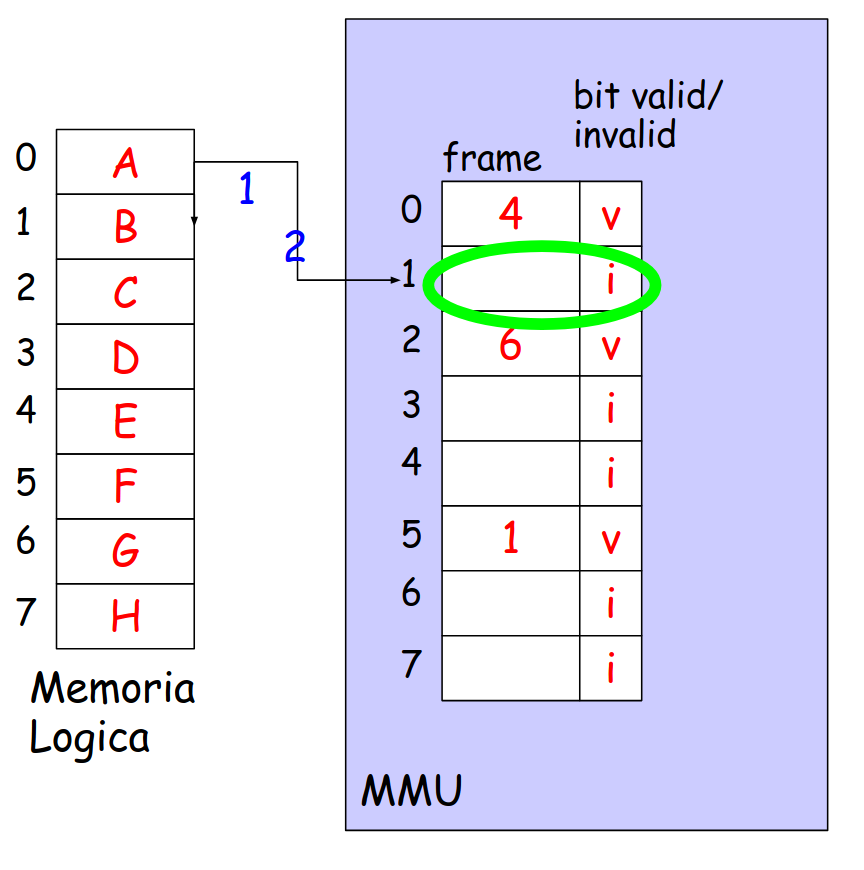
\includegraphics[width=0.3\linewidth]{Images/Screenshot 2025-01-17 at 16-51-24 so-05-memoria - so-05-memoria.pdf.png}
    \end{figure}


3. Viene generato un trap "page fault", che viene catturato dal s.o.
    \begin{figure} [h]
    \centering
    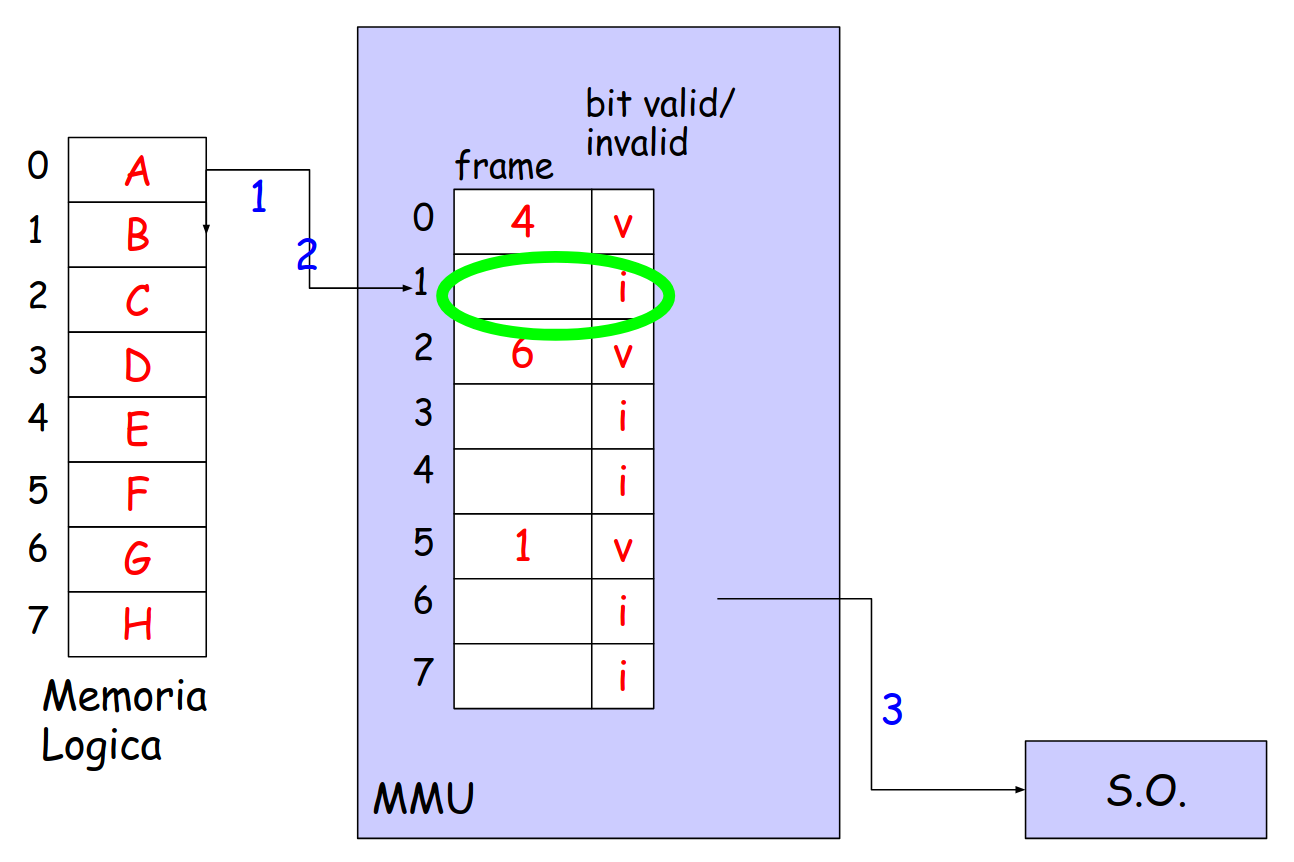
\includegraphics[width=0.45\linewidth]{Images/Screenshot 2025-01-17 at 16-53-05 so-05-memoria - so-05-memoria.pdf.png}
    \end{figure}

\newpage
4. Il s.o. cerca in memoria secondaria la pagina da caricare.
    \begin{figure} [h]
        \centering
        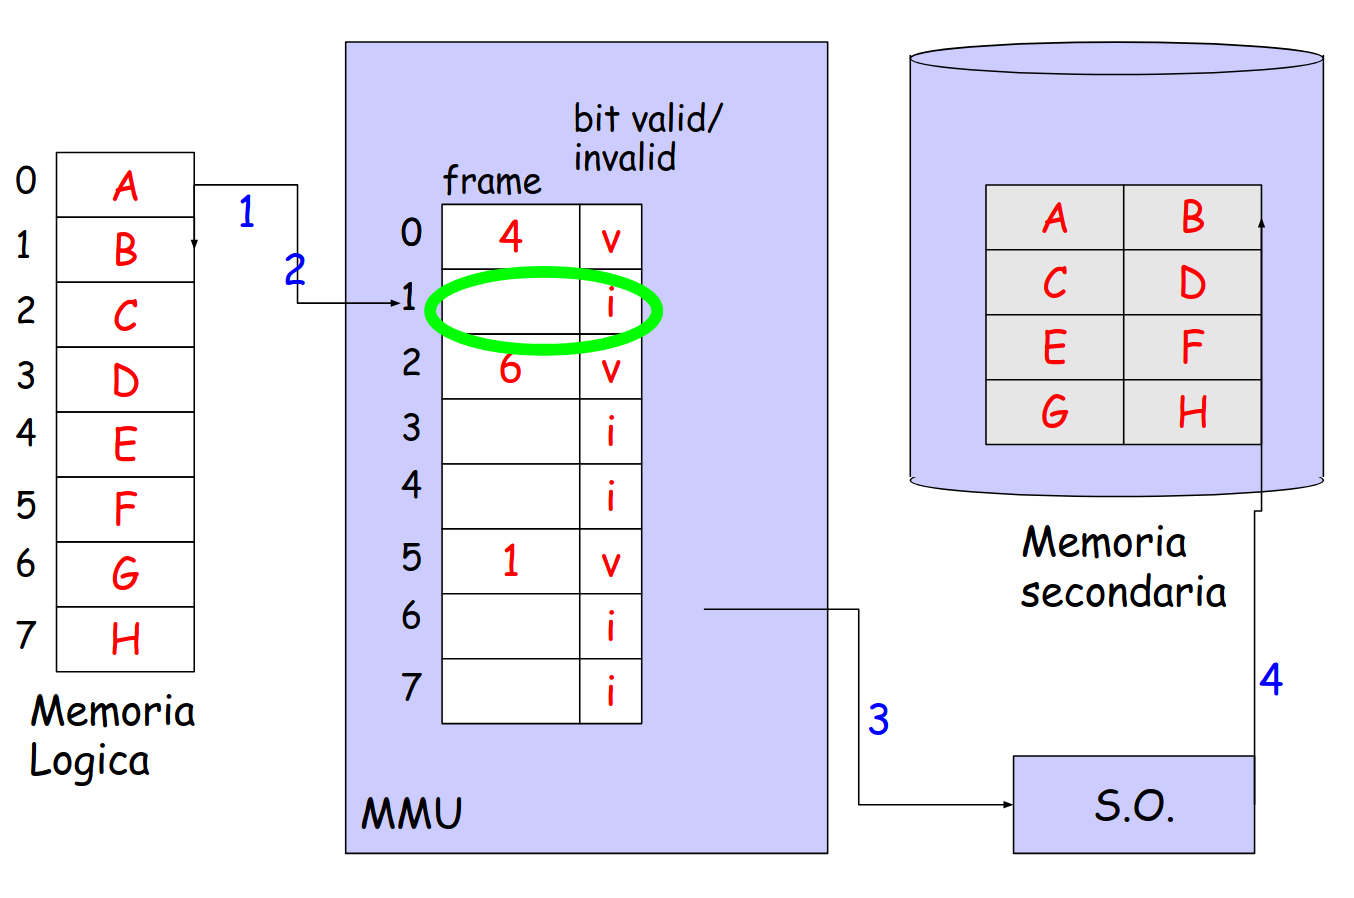
\includegraphics[width=0.4\linewidth]{Images/Screenshot 2025-01-17 at 16-54-12 so-05-memoria - so-05-memoria.pdf.png}
    \end{figure}


5. Il s.o. carica la memoria principale con il contenuto della pagina.

    \begin{figure} [h]
        \centering
        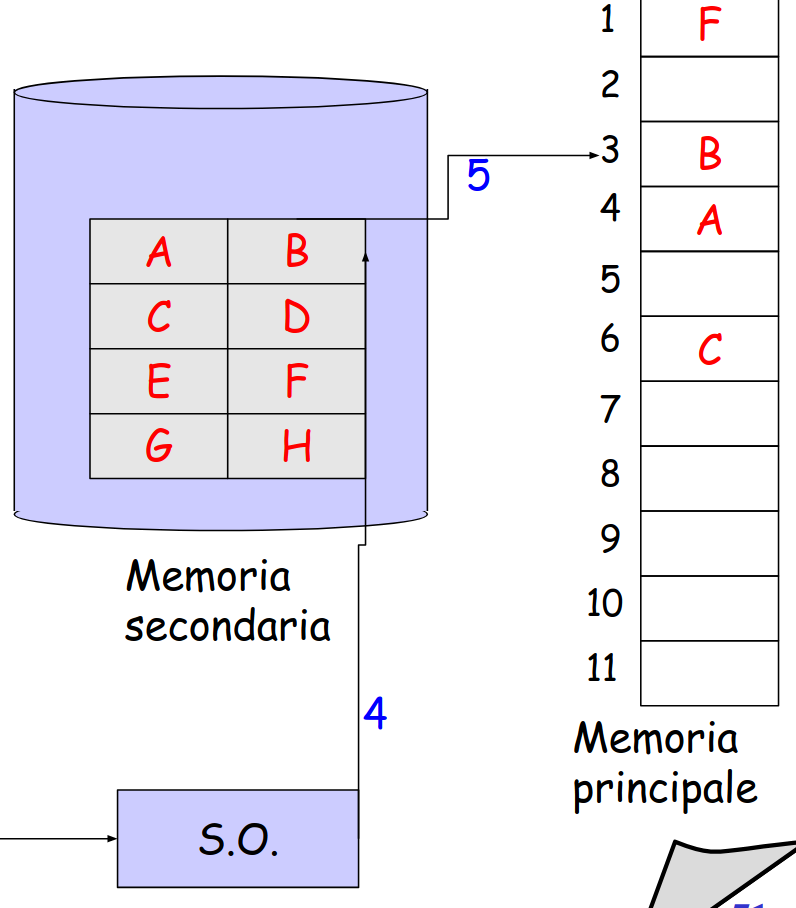
\includegraphics[width=0.3\linewidth]{Images/Screenshot 2025-01-17 at 16-56-21 so-05-memoria - so-05-memoria.pdf.png}
    \end{figure}




6. Il s.o. aggiorna la page table in modo opportuno e riavvia l'esecuzione.

    \begin{figure} [h]
        \centering
        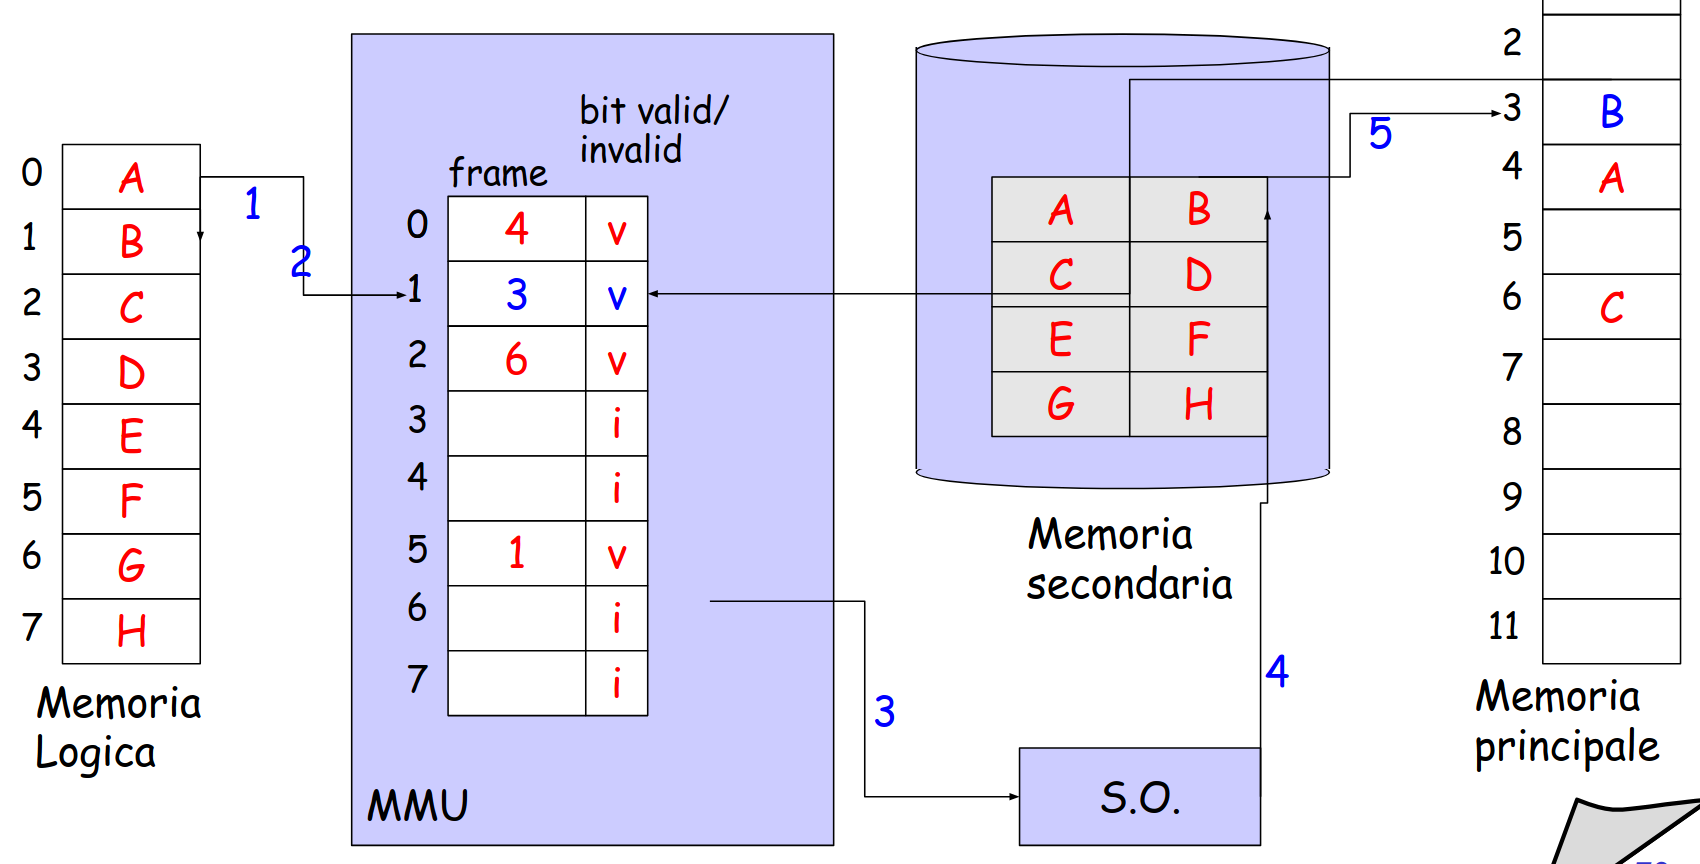
\includegraphics[width=0.6\linewidth]{Images/Screenshot 2025-01-17 at 16-57-37 so-05-memoria - so-05-memoria.pdf.png}
    \end{figure}


In mancanza di frame liberi occorre "liberarne" uno, la pagina da rimpiazzare deve essere la meno "utile".
Esistono \textbf{algoritmi di sostituzione o rimpiazzamento} per questo compito.

\newpage
\subsection{Algoritmo del meccanismo di demand paging}
\begin{itemize}
    \item Individua la pagina in memoria secondaria
    \item Individua un frame libero
    \item Se non esiste un frame libero
        \begin{itemize}
            \item richiama algoritmo di rimpiazzamento
            \item aggiorna la tabella delle pagine (invalida pagina "vittima")
            \item se la pagina "vittima" è stata variata, scrive la pagina sul disco
            \item aggiorna la tabella dei frame (frame libero)
        \end{itemize}
    \item Aggiorna la tabella dei frame (frame occupato)
    \item Leggi la pagina da disco (quella che ha provocato il fault)
    \item Aggiorna la tabella delle pagine
    \item Riattiva il processo
\end{itemize}

\subsection{Algoritmi di rimpiazzamento}
L'algoritmo di rimpiazzamento ha come obiettivo minimizzare il numero di page fault.
Gli algoritmi vengono valutati esaminando come si comportano
quando applicati ad una stringa di riferimenti in memoria.

Stringhe di riferimenti possono essere generate esaminando il funzionamento di programmi reali o con un generatore di numeri random. La stringa di riferimenti può essere limitata ai numeri di pagina, in quanto non siamo interessati agli offset.

Andamento dei page fault in funzione del numero di frame.
Ci si aspetta un grafo monotono decrescente, ma non sempre è così.

\begin{figure} [h]
    \centering
    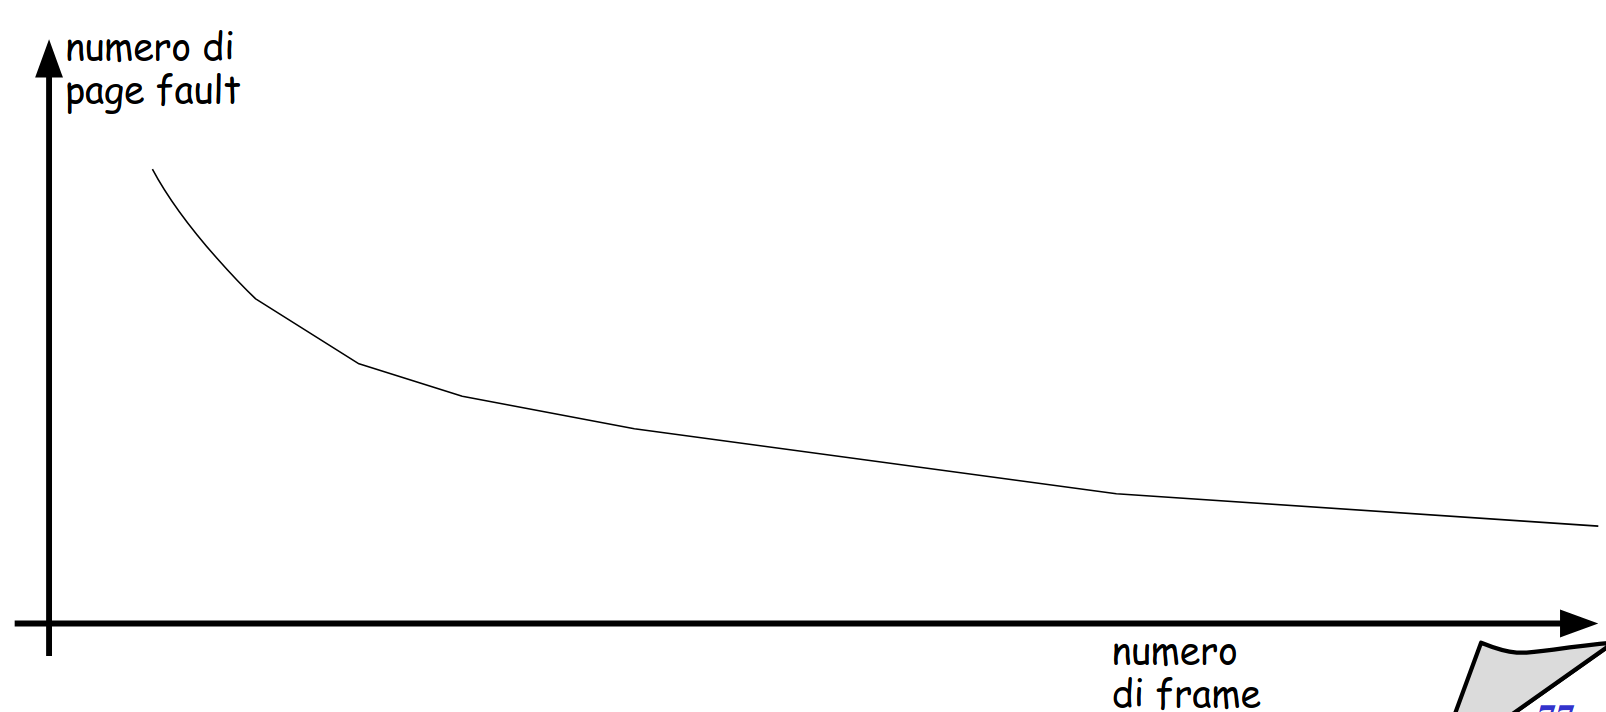
\includegraphics[width=0.7\linewidth]{Images/Screenshot 2025-01-17 at 17-37-53 so-05-memoria - so-05-memoria.pdf.png}
\end{figure}

\subsubsection{Algoritmo FIFO}
\paragraph{Descrizione:}Quando c’è necessità di liberare un frame viene individuato come “vittima” il frame che per primo fu caricato in memoria.

\paragraph{Vantaggi: }semplice, non richiede particolari supporti hardware.
\paragraph{Svantaggi:} vengono talvolta scaricate pagine che sono sempre utilizzate.

\subparagraph{Esempio 1}
numero di frame in memoria: 3 , numero di page fault: 15 (su 20 accessi in memoria)

\begin{figure} [h]
    \centering
    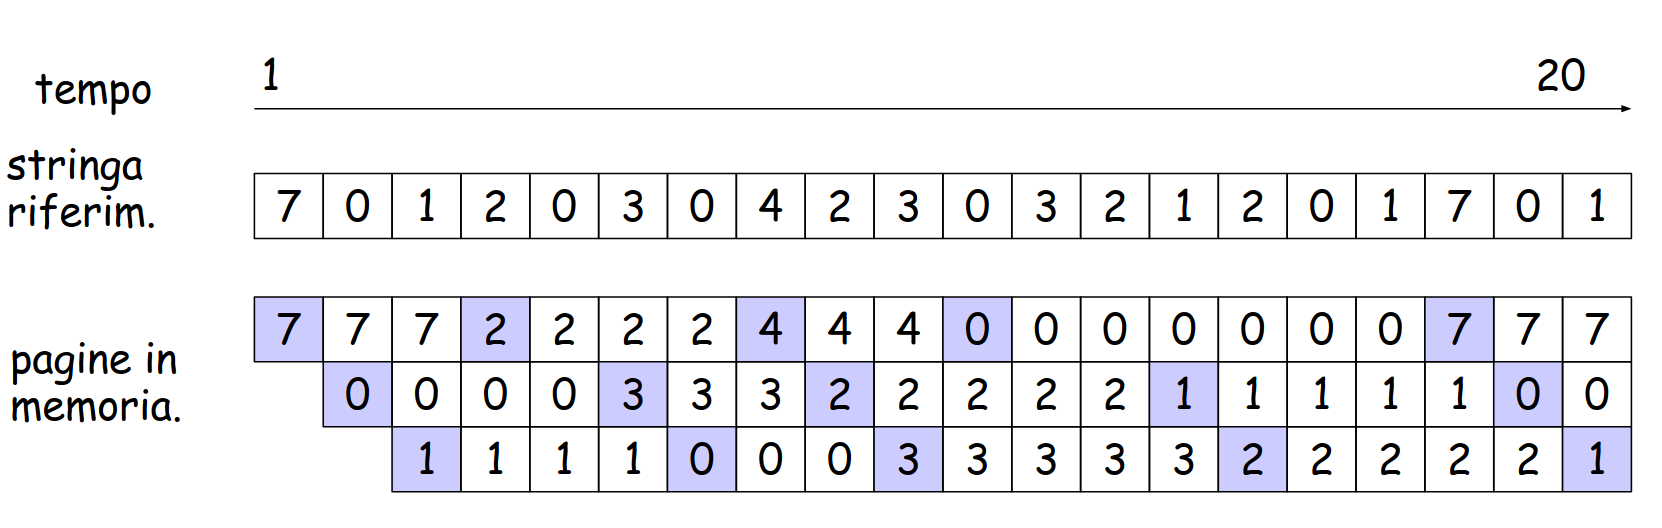
\includegraphics[width=0.8\linewidth]{Images/Screenshot 2025-01-17 at 17-41-02 so-05-memoria - so-05-memoria.pdf.png}
\end{figure}

\newpage

\subparagraph{Esempio 2}
numero di frame in memoria: 3, numero di page fault: 9 (su 12 accessi in memoria)

\begin{figure} [h]
    \centering
    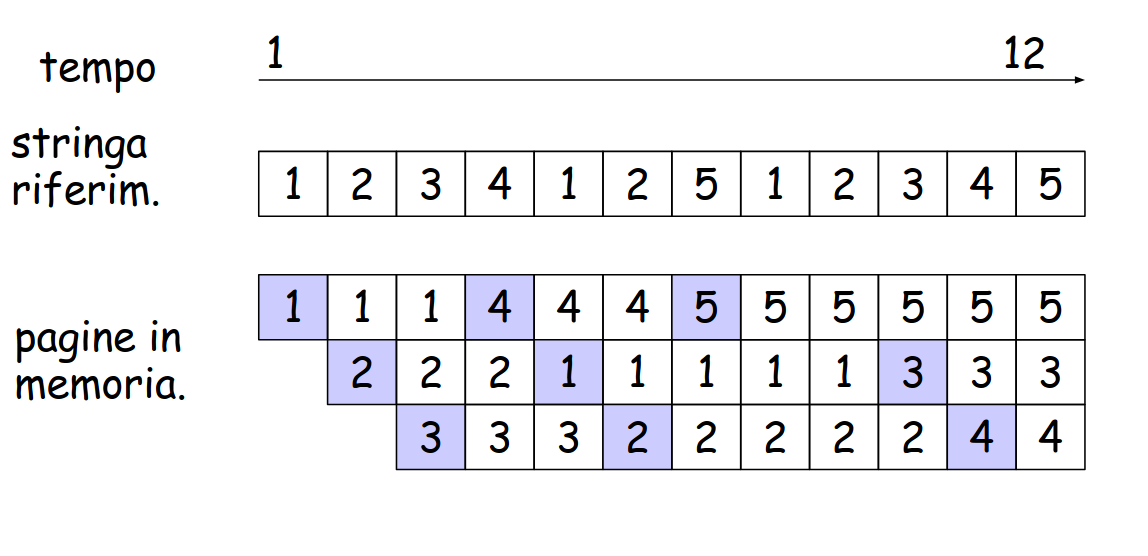
\includegraphics[width=0.65\linewidth]{Images/Screenshot 2025-01-17 at 17-42-55 so-05-memoria - so-05-memoria.pdf.png}
\end{figure}


\subparagraph{Esempio 3}
numero di frame in memoria: 4, numero di page fault: 10 (su 12 accessi in memoria)

\begin{figure} [h]
    \centering
    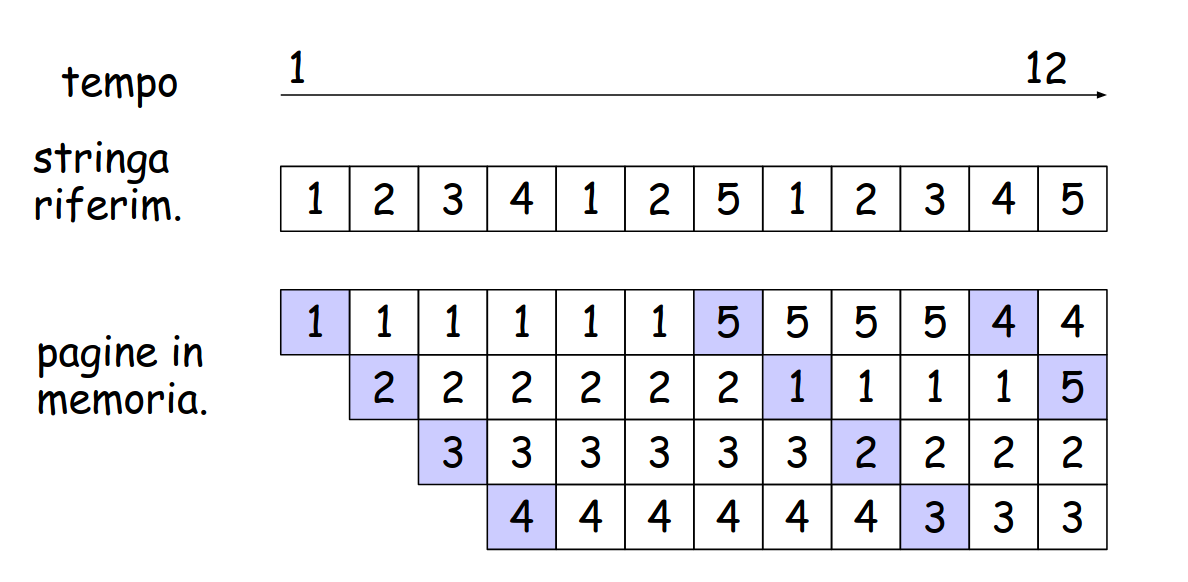
\includegraphics[width=0.65\linewidth]{Images/Screenshot 2025-01-17 at 17-44-49 so-05-memoria - so-05-memoria.pdf.png}
\end{figure}

In alcuni algoritmi di rimpiazzamento non è detto che aumentando il numero di frame allora il numero di page fault diminuisca (e.g., FIFO).
Questo fenomeno indesiderato si chiama \textbf{Anomalia di Belady}.

\begin{figure} [h]
    \centering
    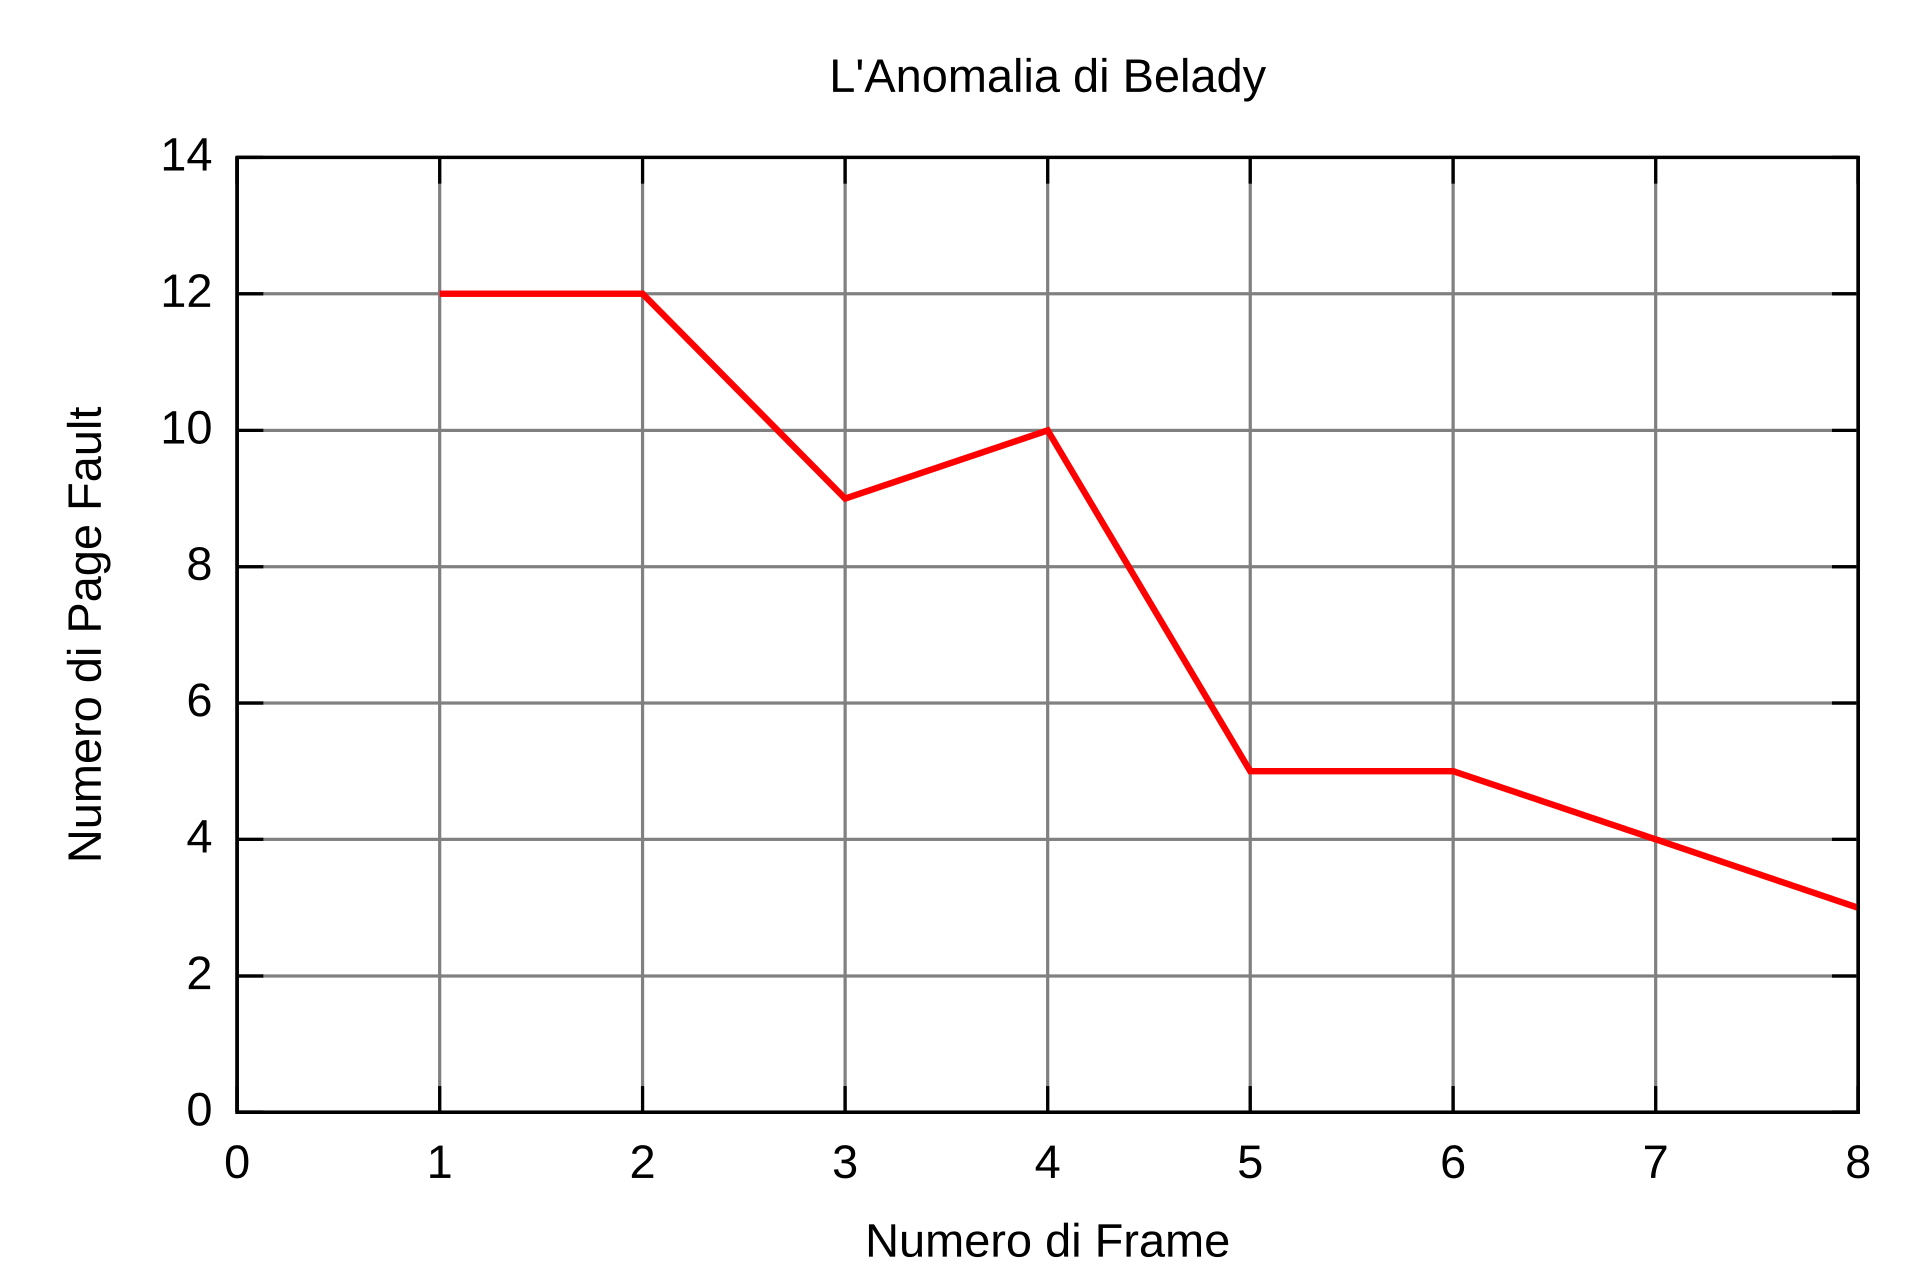
\includegraphics[width=0.65\linewidth]{Images/Anomalia_di_Belady.svg.png}
\end{figure}
\newpage
\subsubsection{Algoritmo MIN - Ideale}
\paragraph{Descrizione:} seleziona come pagina vittima una pagina che non sarà più acceduta o la pagina che verrà acceduta nel futuro più lontano.

Ottimale perché fornisce il minimo numero di page fault, è un \textbf{algoritmo teorico} perché richiederebbe la conoscenza a priori della stringa dei riferimenti futuri del programma,
viene utilizzato a posteriori come paragone per verificare le
performance degli algoritmi di rimpiazzamento reali.

\subparagraph{Esempio}
numero di frame in memoria: 3, numero di page fault: 9 (su 20 accessi in memoria)

\begin{figure} [h]
    \centering
    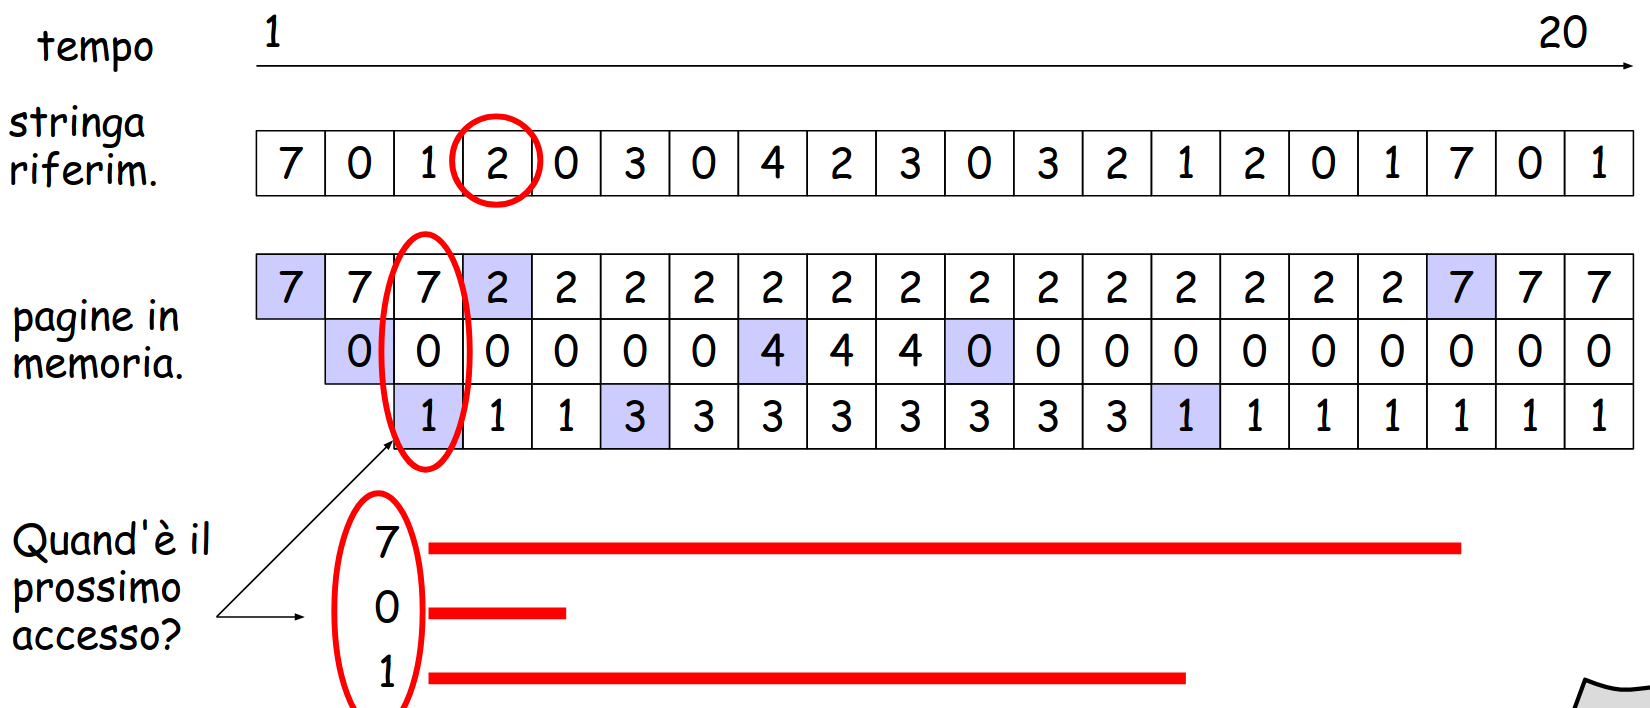
\includegraphics[width=0.7\linewidth]{Images/Screenshot 2025-01-17 at 17-53-59 so-05-memoria - so-05-memoria.pdf.png}
\end{figure}

\subsection{Algoritmo LRU (Least Recently Used)}
\paragraph{Descrizione:} seleziona come pagina vittima la pagina che è stata usata meno recentemente nel passato.

Basato sul presupposto che la distanza tra due riferimenti successivi alla stessa pagina non vari eccessivamente, stima la distanza nel futuro utilizzando la distanza nel passato.

\subparagraph{Esempio}
numero di frame in memoria: 3, numero di page fault: 12 (su 20 accessi in memoria)

\begin{figure} [h]
    \centering
    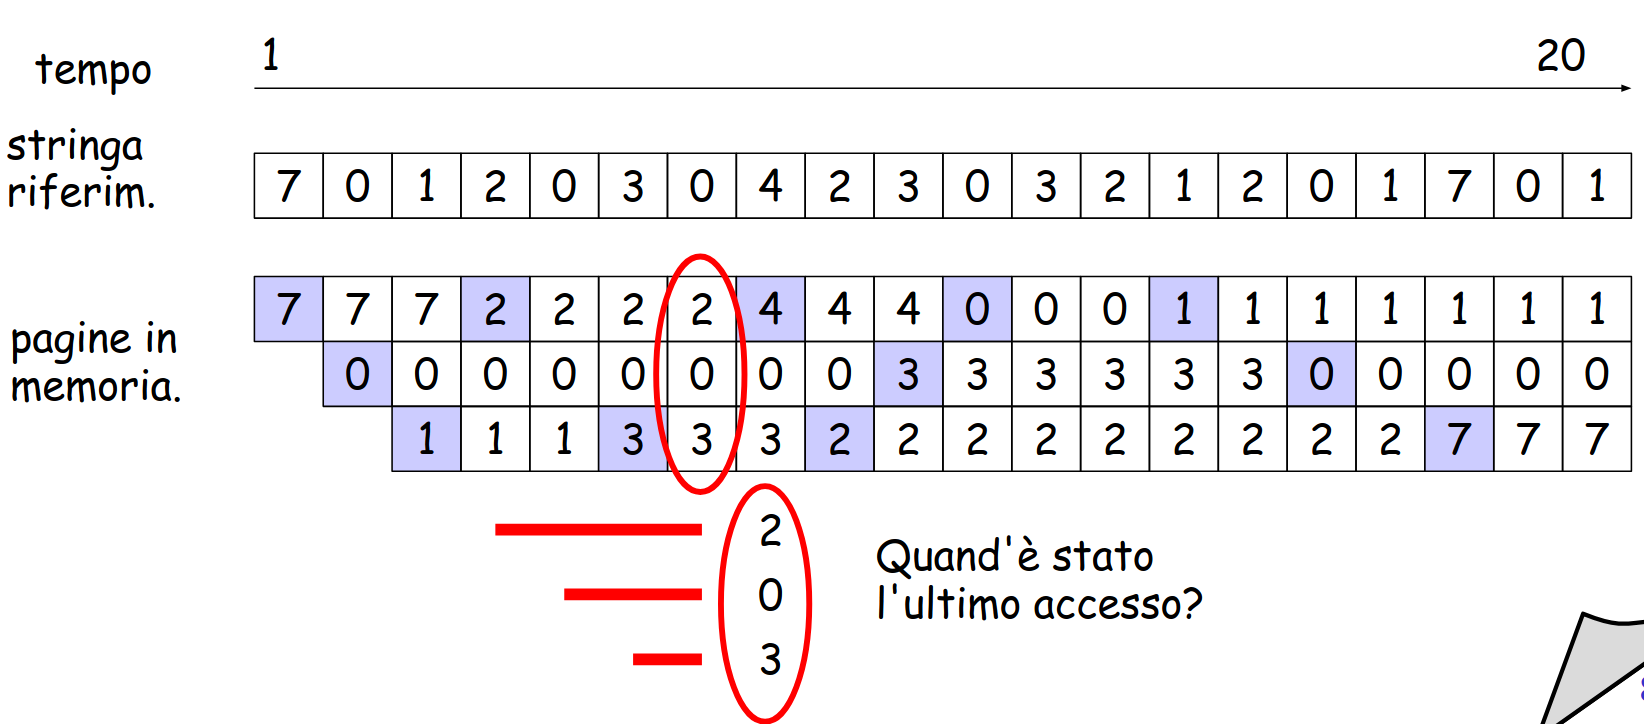
\includegraphics[width=0.7\linewidth]{Images/Screenshot 2025-01-17 at 17-56-57 so-05-memoria - so-05-memoria.pdf.png}
\end{figure}

\paragraph{Implementazione:} E' necessario uno specifico supporto hardware.
La MMU deve registrare nella tabella delle pagine un \textbf{time-stamp} quando accede ad una pagina. Il time-stamp può essere implementato come un contatore che viene incrementato ad ogni accesso in memoria.

Bisogna gestire l'overflow dei contatori, essi devono essere memorizzati in memoria e questo richiede accessi addizionali alla memoria.
La tabella deve essere scandita totalmente per trovare la
pagina LRU.


\paragraph{Implementazione basata su stack:}
Si mantiene uno stack di pagine, tutte le volte che una pagina viene acceduta, viene rimossa dallo stack (se presente) e posta in cima allo stack stesso.
In questo modo:
\begin{itemize}
    \item in cima si trova la pagina utilizzata più di recente.
    \item in fondo si trova la pagina utilizzata meno di recente.
\end{itemize}

L'aggiornamento di uno stack organizzato come double-linked list richiede l'aggiornamento di 6 puntatori!

La pagina LRU viene individuata con un accesso alla memoria.


\newpage
\subsubsection{Algoritmi a stack}

\paragraph{Definizione:} si indichi con $S_t(A,m)$ l'insieme delle pagine mantenute in memoria centrale al tempo t dell'algoritmo A, data una memoria di m frame.

Un algoritmo a stack non genera casi di Anomalia di Belady. L'algoritmo di LRU è a stack.

\paragraph{}
Un algoritmo di rimpiazzamento viene detto \textbf{stack algorithm} se per ogni istante t si ha: 
\newline
$S_t(A,m) \subseteq S_t(A,m+1)$
\newline
\paragraph{}
In altre parole: se l'insieme delle pagine in memoria con \textbf{m} frame è sempre un sottoinsieme delle pagine in memoria con \textbf{m + 1} frame.

\subsubsection{LRU - Implementazione approssimata}
In entrambi i casi (contatori, stack), mantenere le informazione per LRU è troppo costoso.

In realtà poche MMU forniscono il supporto hardware per l'algoritmo LRU, alcuni sistemi non forniscono alcun tipo di supporto, e in tal caso l'algoritmo FIFO deve essere utilizzato.

\paragraph{Reference bit:} alcuni sistemi forniscono supporto sotto forma di reference bit, tutte le volte che una pagina è acceduta, il bit associato alla pagina viene aggiornato a 1.
\subparagraph{}
Inizialmente, tutti i bit sono posti a zero dal s.o. , durante l'esecuzione dei processi, le pagine in memoria vengono
accedute e i reference bit vengono posti a 1.

Periodicamente, è possibile osservare quali pagine sono state
accedute e quali non osservando i reference bit, ma non conosciamo l'ordine in cui sono state usate.

\paragraph{Additional-Reference-Bit-Algorithm:}
Possiamo aumentare le informazioni di ordine "salvando" i reference bit ad intervalli regolari (ogni 100 ms)

Esempio: manteniamo 8 bit di "storia" per ogni pagina.

Il nuovo valore del reference bit viene salvato tramite shift a destra della storia ed inserimento del bit come most signif. bit

La pagina vittima è quella con valore minore; in caso di parità, si utilizza una disciplina FIFO.

\begin{figure} [h]
    \centering
    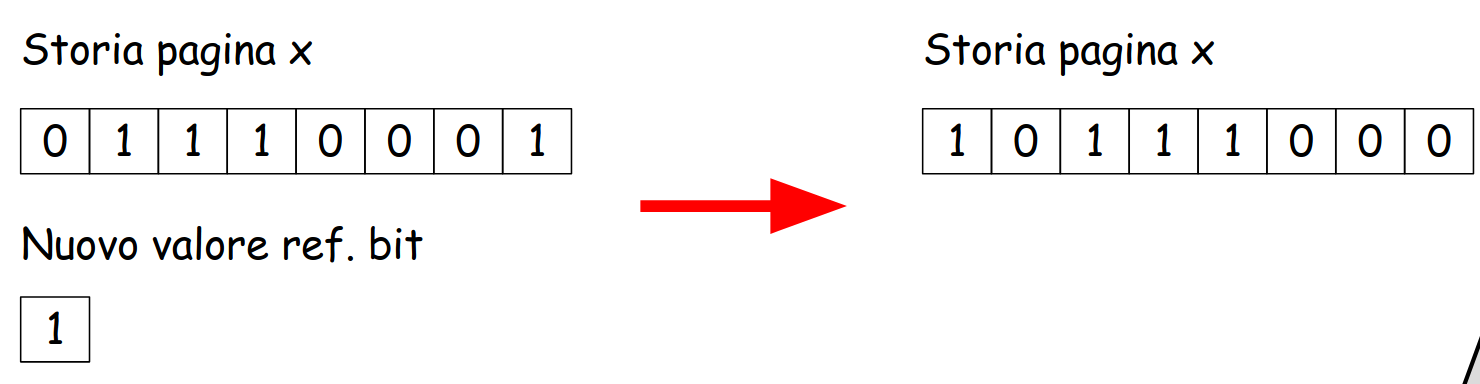
\includegraphics[width=0.7\linewidth]{Images/Screenshot 2025-01-17 at 18-15-39 so-05-memoria - so-05-memoria.pdf.png}
\end{figure}
\newpage
\subsubsection{Second-chance algorithm}
Conosciuto anche come algoritmo dell'orologio, corrisponde ad un caso particolare dell'algoritmo precedente, dove la
dimensione della storia è uguale a 1.

\paragraph{Descrizione:} le pagine in memoria vengono gestite come una lista circolare, a partire dalla posizione successiva all'ultima pagina caricata, si scandisce la lista con la seguente regola:
\begin{itemize}
    \item se la pagina è stata acceduta (reference bit a 1) allora il reference bit viene messo a 0. 
    \item se la pagina non è stata acceduta (reference bit a 0) allora la pagina selezionata è la vittima.
\end{itemize}

L'idea è semplice: l'algoritmo seleziona le pagine in modo FIFO, se però la pagina è stata acceduta, gli si dà una "seconda possibilità" (second chance);

Si cercano pagine successive che non sono state accedute, se tutte le pagine sono state accedute, degenera nel meccanismo FIFO.

L'implementazione è semplice e non richiede capacità complesse da parte della MMU.

\begin{figure} [h]
    \centering
    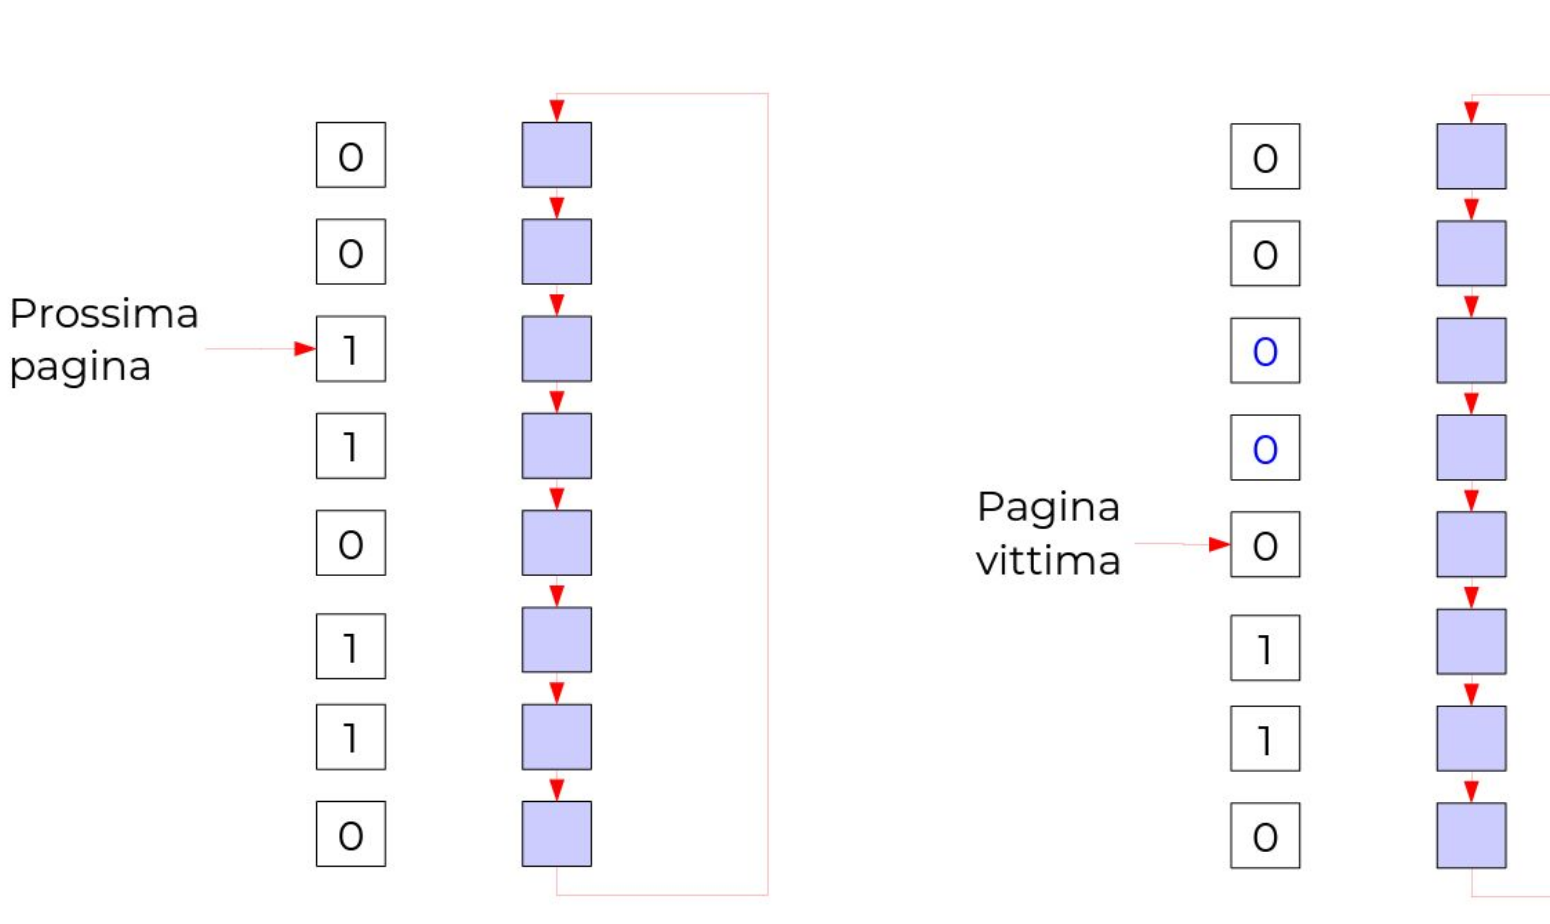
\includegraphics[width=0.7\linewidth]{Images/Screenshot 2025-01-17 at 18-21-08 so-05-memoria - so-05-memoria.pdf.png}
\end{figure}

\subsubsection{Altri algoritmi di rimpiazzamento}
\paragraph{Least frequently used (LFU)} si mantiene un contatore del numero di accessi ad una pagina, la pagina con il valore minore viene scelta come vittima.

Una pagina utilizzata spesso dovrebbe avere un contatore molto alto.

Può essere approssimato tramite reference bit.

\subparagraph{Problemi:} se una pagina viene utilizzata frequentemente all'inizio, e poi non viene più usata, non viene rimossa per lunghi periodi.

\paragraph{Most frequently used (MFU)}
si mantiene un contatore del numero di accessi ad una pagina, la pagina con il valore maggiore viene scelta come vittima

Pagine appena caricate hanno un valore molto basso, e non dovrebbero essere rimosse.

Può essere approssimato tramite reference bit

\subparagraph{Problemi:} problemi di performance.

\subsection{Allocazione}
Con algoritmo di allocazione (per memoria virtuale) si intende l'algoritmo utilizzato per scegliere quanti frame assegnare ad ogni
singolo processo.

\paragraph{Allocazione locale} ogni processo ha un insieme proprio di frame, poco flessibile.

\paragraph{Allocazione globale} tutti i processi possono allocare tutti i frame presenti nel sistema (sono in competizione), può portare a \textbf{trashing}.

\subsubsection{Trashing}
\paragraph{Definizione:} un processo (o un sistema) si dice che è in trashing quando spende più tempo per la paginazione che per l'esecuzione.

Le possibili cause in un sistema con allocazione globale: si ha trashing se i processi tendono a "rubarsi i frame a vicenda",
ovvero non riescono a tenere in memoria i frame utili a breve termine, perchè altri processi chiedono frame liberi e quindi generano page fault ogni pochi passi di avanzamento.

\subparagraph{Esempio}
esaminiamo un sistema che accetti nuovi processi quando il grado di
utilizzazione della CPU è basso. Se per qualche motivo gran parte dei processi entrano in page fault:
\begin{itemize}
    \item la ready queue si riduce
    \item il sistema sarebbe indotto ad accettare nuovi processi
\end{itemize}
E' UN ERRORE!

Statisticamente, il sistema: genererà un maggior numero di page fault e di conseguenza diminuirà il livello della multiprogrammazione.

\begin{figure} [h]
    \centering
    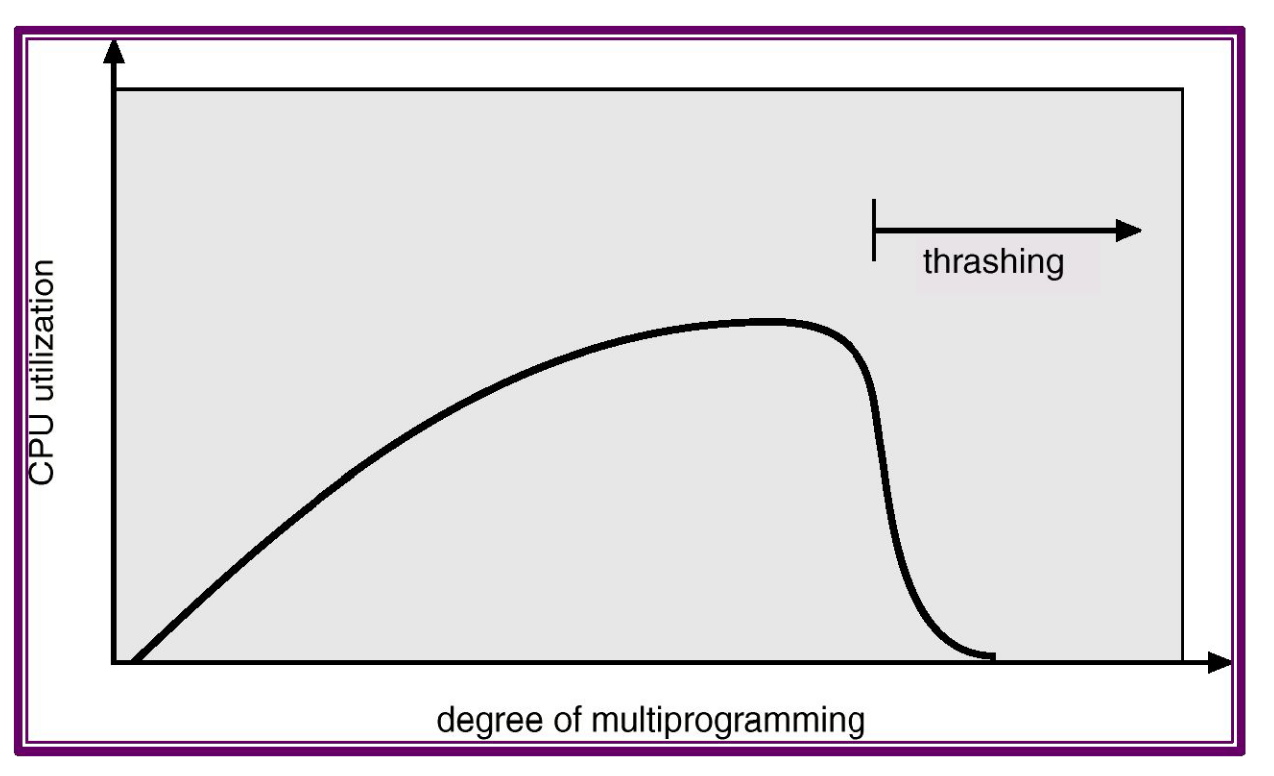
\includegraphics[width=0.6\linewidth]{Images/Screenshot 2025-01-17 at 18-33-00 so-05-memoria - so-05-memoria.pdf.png}
\end{figure}

\subsubsection{Working Set}
\paragraph{Definizione:} si definisce \textbf{working set} di finestra $\Delta$ l'insieme delle pagine accedute nei più recenti $\Delta$ riferimenti.

E' una rappresentazione approssimata del concetto di località, se una pagina non compare in $\Delta$ riferimenti successivi in memoria, allora esce dal working set; non è più una pagina su cui si lavora attivamente.
\newline


Esempio con $\Delta$ = 5

\begin{figure} [h]
        \centering
        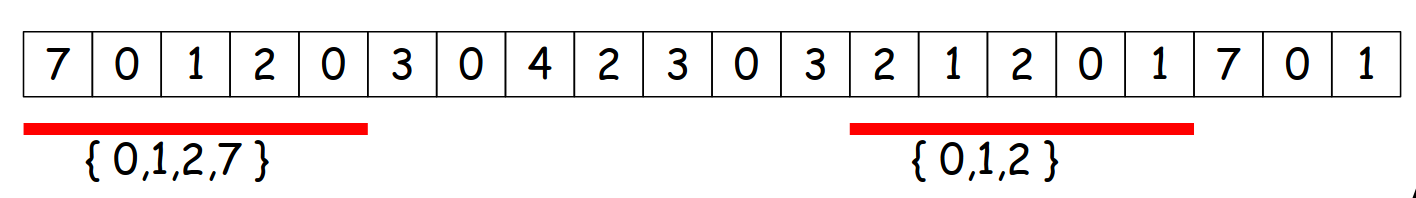
\includegraphics[width=0.6\linewidth]{Images/Screenshot 2025-01-17 at 18-38-59 so-05-memoria - so-05-memoria.pdf.png}
    \end{figure}


Se si sceglie $\Delta$ troppo piccolo: si considera non più utile ciò che in realtà serve. 

Minore inerzia nel "buttare via".

Se si sceglie $\Delta$ troppo grande: si considera utile anche ciò che non serve più. 

Sistema più "conservatore".

\paragraph{Cosa serve il Working Set?}
Se l'ampiezza della finestra è ben calcolata, il working set è una
buona approssimazione dell'insieme delle pagine "utili".

Sommando quindi l'ampiezza di tutti i working set dei processi
attivi, questo valore deve essere sempre minore del numero di
frame disponibili, altrimenti il sistema è in trashing.

\paragraph{Come si usa il Working Set?}
Serve per controllare l'allocazione dei frame ai singoli processi. 

Quando ci sono sufficienti frame disponibili non occupati dai
working set dei processi attivi, allora si può attivare un nuovo
processo.

Se al contrario la somma totale dei working set supera il numero totale dei frame, si può decidere di sospendere l'esecuzione di un processo.

